 %%%%%%%%%%%%%%%%%%%%%%%%%
% Dokumentinformationen %
%Dokumentinformationen	======================================================================

\newcommand{\titleinfo}{IntTra}
\newcommand{\authorinfo}{Dev4Future, sowie weitere Autoren}
\newcommand{\versioninfo}{HS / 2019}

%weitere Autoren: ==========================================================================
%Dev4Future, Braun \& Co, Jürg \& Co, Hannes, Körner, Gwerder, Niedermann

%%%%%%%%%%%%%%%%%%%%%%%%%%%%%%%%%%%%%%%%%%%%%
% Standard projektübergreifender Header für
% - Makros 
% - Farben
% - Mathematische Operatoren
%
% DORT NUR ERGÄNZEN, NICHTS LÖSCHEN
%%%%%%%%%%%%%%%%%%%%%%%%%%%%%%%%%%%%%%%%%%%%%
% Dokumenteinstellungen	 ======================================================================
% Genereller Header
\documentclass[10pt,twoside,a4paper,fleqn]{article}
% Dateiencoding
\usepackage[utf8]{inputenc}
% Seitenränder
\usepackage[left=1cm,right=1cm,top=1cm,bottom=1cm,includeheadfoot]{geometry}
% Sprachpaket
\usepackage[ngerman]{babel,varioref}

% Pakete
\usepackage{amssymb,amsmath,fancybox,graphicx,lastpage,wrapfig,fancyhdr,hyperref,verbatim,floatflt,multicol,multirow,rotating,pdflscape,array,longtable,listings}

% Zum Bilder einfach in Tabellen einfügen (valign=t)
\usepackage[export]{adjustbox}

%%%%%%%%%%%%%%%%%%%%
% Generelle Makros %
%%%%%%%%%%%%%%%%%%%%
\newcommand{\skript}[1]{$_{\textcolor{red}{\mbox{\small{Skript S.#1}}}}$}
\newcommand{\verweis}[2]{\small{(siehe auch \ref{#1}, #2 (S. \pageref{#1}))}}
\newcommand{\verweiskurz}[1]{(\small{siehe \ref{#1}\normalsize)}}
\newcommand{\subsubadd}[1]{\textcolor{black}{\mbox{#1}}}
\newcommand{\formelbuch}[1]{$_{\textcolor{red}{\mbox{\small{S#1}}}}$}

\newcommand{\kuchling}[1]{$_{\textcolor{red}{\mbox{\small{Kuchling #1}}}}$}
\newcommand{\stoecker}[1]{$_{\textcolor{orange}{\mbox{\small{Stöcker #1}}}}$}
\newcommand{\sachs}[1]{$_{\textcolor{blue}{\mbox{\small{Sachs S. #1}}}}$}
\newcommand{\hartl}[1]{$_{\textcolor{green}{\mbox{\small{Hartl S. #1}}}}$}

\newcommand{\schaum}[1]{\tiny Schaum S. #1}

\newcommand{\skriptsection}[2]{\section{#1 {\tiny Skript S. #2}}}
\newcommand{\skriptsubsection}[2]{\subsection{#1 {\tiny Skript S. #2}}}
\newcommand{\skriptsubsubsection}[2]{\subsubsection{#1 {\tiny Skript S. #2}}}

\newcommand{\matlab}[1]{\footnotesize{(Matlab: \texttt{#1})}\normalsize{}}

%%%%%%%%%%
% Farben %
%%%%%%%%%%
\usepackage{xcolor}

%%%%%%%%%%%%%%%%%%%%%%%%%%%%
% Mathematische Operatoren %
%%%%%%%%%%%%%%%%%%%%%%%%%%%%
\DeclareMathOperator{\sinc}{sinc}
\DeclareMathOperator{\sgn}{sgn}
\DeclareMathOperator{\Real}{Re}
\DeclareMathOperator{\Imag}{Im}
%\DeclareMathOperator{\e}{e}
\DeclareMathOperator{\cov}{cov}
\DeclareMathOperator{\PolyGrad}{PolyGrad}

%Makro für 'd' von Integral- und Differentialgleichungen 
\newcommand*{\diff}{\mathop{}\!\mathrm{d}}


%%%%%%%%%%%%%%%%%%%%%%%%%%%
% Fouriertransformationen %
%%%%%%%%%%%%%%%%%%%%%%%%%%%
\usepackage{trfsigns, trsym}
%\unitlength1cm
% Zeitbereich -- Frequenzbereich
%\newcommand{\laplace}
%{
%\begin{picture}(1,0.5)
%\put(0.2,0.1){\circle{0.14}}\put(0.27,0.1){\line(1,0){0.5}}\put(0.77,0.1){\circle*{0.14}}
%\end{picture}
%}
% Frequenzbereich -- Zeitbereich
%\newcommand{\Laplace}
%{
%\begin{picture}(1,0.5)
%\put(0.2,0.1){\circle*{0.14}}\put(0.27,0.1){\line(1,0){0.45}}\put(0.77,0.1){\circle{0.14}}
%\end{picture}
%}


% Fouriertransformationen
\unitlength1cm
\newcommand{\FT}
{
\begin{picture}(1,0.5)
\put(0.2,0.1){\circle{0.14}}\put(0.27,0.1){\line(1,0){0.5}}\put(0.77,0.1){\circle*{0.14}}
\end{picture}
}


\newcommand{\IFT}
{
\begin{picture}(1,0.5)
\put(0.2,0.1){\circle*{0.14}}\put(0.27,0.1){\line(1,0){0.45}}\put(0.77,0.1){\circle{0.14}}
\end{picture}
}




%%%%%%%%%%%%%%%%%%%%%%%%%%%%
% Allgemeine Einstellungen %
%%%%%%%%%%%%%%%%%%%%%%%%%%%%
%PDF Info
\hypersetup{pdfauthor={\authorinfo},pdftitle={\titleinfo},colorlinks=false}
\author{\authorinfo}
\title{\titleinfo}

%%%%%%%%%%%%%%%%%%%%%%%
% Kopf- und Fusszeile %
%%%%%%%%%%%%%%%%%%%%%%%
\pagestyle{fancy}
\fancyhf{}
%Linien oben und unten
\renewcommand{\headrulewidth}{0.5pt} 
\renewcommand{\footrulewidth}{0.5pt}

\fancyhead[L]{\titleinfo{ }\tiny{(\versioninfo)}}
%Kopfzeile rechts bzw. aussen
\fancyhead[R]{Seite \thepage { }von \pageref{LastPage}}
%Fusszeile links bzw. innen
\fancyfoot[L]{\footnotesize{\authorinfo}}
%Fusszeile rechts bzw. ausen
\fancyfoot[R]{\footnotesize{\today}}
%Lizenz CC-BY-NC-SA
% Headerfile für die Einbindung einer Lizenzgrafik in den Footer
% Verwendung: \lizenz{cc-by-nc-sa}{small}
\newcommand{\lizenz}[2]
{
\fancyfoot[C]{
  \includegraphics[width=1.6cm]{./header/lizenzen/#1/#2.png}
}
}
\lizenz{cc-by-nc-sa}{small}
%Einrücken verhindern versuchen
\setlength{\parindent}{0pt}

% Zeilenhöhe Tabellen:
\newcommand{\arraystretchOriginal}{1.5}
\renewcommand{\arraystretch}{\arraystretchOriginal}

			% standard header mit den Packages includieren



% Sections ======================================================================
%TODO ersetzen von Bildern mit richtigem Latex Code (Kap 3.1 und 5.3.1) 
\begin{document}
		% Einleitung/ Varianten der Integraltransformationen
		\section{Varianten der Integraltransformationen } %\skript{55}
	\begin{tabular}{|l||l|l|}
	\hline
	\textbf{Signalart}
		& diskret
		& kontinuierlich \\
	\hline \hline
	periodisch
		& Diskrete Fourier-Transformation
		& Fourierreihe \\
	\hline
	diskret/ impulsförmig
		& ``Fourierreihe mit $T = Impulsdauer$''
		& Fourierintegral \\
	\hline
	kausal
		& Z-Transformation
		& Laplace-Transformation \\Bronstein
	\hline
	\end{tabular}
		
		% Signale und Systeme
		\section{Signale und Systeme}
	\begin{tabular}{|l|l|}
    	\hline
    	\textbf{Linearität} & \textbf{Zeitinvarianz}\\
    	\hline
    	$S(x1+x2)=S(x1)+S(x2)$ & $S(x(t-t_0)=S(x)\cdot x(t-t_0)$ \\
    	$S(c\cdot x)=c\cdot S(x)$ & \\
		\hline    
    \end{tabular}
  	
	\subsection{Lineare Systeme}
		\textbf{Basissignale}
		\begin{list}{$\bullet$}{\setlength{\itemsep}{0cm} \setlength{\parsep}{0cm} \setlength{\topsep}{0cm}} 
          \item Lineare Systeme sind durch die Antworten auf die
          Basissignale bestimmt.
          \item Basissignale müssen linear unabhängig voneinander sein, d.h. ein
		Basissignal darf nicht durch \textbf{Linearkombination} anderer Basissignale
		darstellbar sein          
		  \item Alle möglichen Eingangs-Funktionen müssen durch eine Linearkombination der
		Basissignale dargestellt werden können. $\Rightarrow$ \textbf{Periode des Eingangssignals =	Anzahl Basissignale}
        \end{list}
        \vspace{.2cm}
		\textbf{Berechnung der Systemantwort aufgrund der Basissignale und der
		Anregung}\\
		1. Eingangssignal $x$ als Linearkombination der Basisvektoren darstellen
		$\Rightarrow$ lineares Gleichungssystem\\
		$\Rightarrow x=r\cdot a + s\cdot b + t\cdot c\qquad$ ($x=$
		Eingangssignal; $a,b,c=$ Basisvektoren; $r,s,t=$
		Linearkombinationsparameter)\\ 
		2. Systemantwort $y=r\cdot S(a) + s\cdot S(b) + t\cdot S(c); \qquad (S(a)=$
		Systemantwort der Basis $a$)
	
	\subsection{Lineare zeitinvariante Systeme (LTI-Systeme)}
		LTI-Systeme sind durch ihre Impulsantwort $h$ vollständig bestimmt\\ \\
		\textbf{Berechnung der Systemantwort von diskreten LTI-Systemen}\\
		$\; y=x*h \qquad$ ($y=$ Systemantwort; $x=$ Eingangssignal; $h=$
		Impulsantwort)\\
		
		\textbf{Berechnung der Systemantwort von kontinuierlichen LTI-Systemen}\\
		\begin{tabular}{ll}
			\parbox{8cm}{
			$$s_2(t) = h(t) * s_1(t) \laplace S_2(s) = H(s) S_1(s)$$
			$$h(t) \laplace H(s)$$}
			& \parbox{4cm}{
			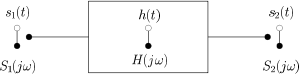
\includegraphics[width=5cm]{./bilder/utf-theorie.png}}\\
		\end{tabular}	
		
	\subsection{Faltung}
	$y(t) = f(t)\ast g(t) = g(t) \ast f(t) = (f \ast g)(t) :=
	\int\limits_{-\infty}^\infty f(u) \cdot g(t-u)\,du =
	\int\limits_{-\infty}^\infty f(t-u) \cdot h(u)\,du $ \\
	wobei gilt: $h\left/t\right) g(t) = $ Impulsantwort des Systems \\
	Hat $g\left(t\right)$ keine negative Argumente dann gilt :
	$\left(g \ast f \right)\left(t\right)=\int\limits_{-\infty}^t f(u) \cdot
	g(t-u)\,du$\\
	Hat $f\left(t\right)$ keine negative Argumente (Einschaltvorgang) dann gilt :
	$\left(g \ast f \right)\left(t\right)=\int\limits_{0}^t f(u) \cdot
	g(t-u)\,du$\\
	Bei einer Faltung mit einer $\delta\left(t\right)$Funktion
	gilt:$f\left(t\right) \ast \delta\left(t\right) = f\left(t\right)$\\
	
	\newpage
	
	\begin{multicols}{2}
		\textbf{grafische Interpretation:}
		\begin{enumerate}
  			\item einfacheres Signal an der Y-Achse spiegeln
  			\item Verschiebung um t nach rechts
  			\item Multiplikation und Integration der beiden Signale
		\end{enumerate}
		\columnbreak
		\textbf{Bestimmung der Grenzen:}
		\begin{enumerate}
		  \item Koordinatensystem: X-Achse: t, Y-Achse: u
		  \item Erster Faktor $\rightarrow$ Streifen parallel zur X-Achse
		  \item Zweiter Faktor $\rightarrow$ Streiffen parallel zur $45^{\circ}$-Geraden
		  \item Grenzen für ein bestimmtes t ablesen
		\end{enumerate}
	\end{multicols}	


		
		% Diskrete Fourier Transformation
		%\section{Diskrete Fourier Transformation (DFT)}
	$$\boxed{s(h)=\sum_{k=0}^{N-1}\hat c_k e^{jhk\frac{2\pi}{N}}=\sum_{k=0}^{N-1}
	\left[ \hat{a}_k \cos\left(hk \frac{2 \pi}{N}\right)+\hat{b}_k \sin\left(hk
	\frac{2 \pi}{N}\right) \right]} \qquad N=\text{Periodenanzahl}$$\\
	$$\hat{c}_k=\frac{1}{N}\sum_{h=0}^{N-1}s(h)
	e^{-jhk\frac{2\pi}{N}}=\hat{a}_k-j\hat{b}_k \qquad \hat{a}_k=\frac{1}{N}
	\sum_{h=0}^{N-1}s(h) \cos\left(hk \frac{2 \pi}{N}\right)=Re(\hat{c}_k) \qquad
	\hat{b}_k=\frac{1}{N} \sum_{h=0}^{N-1}s(h) \sin\left(hk \frac{2
	\pi}{N}\right)=-Im(\hat{c}_k)$$\\	

	\subsection{Berechnung mit Matrizen}
		\textbf{Transformation}\\
		1. Periode $N$ des Signalvektors $\vec{s}=
		\begin{bmatrix}
		s(0) \\
		s(1) \\
		s(N-1)\\
		\end{bmatrix}$ bestimmen\\ \\
		2. Einheitswurzel $w$ berechnen: $w=e^{j\frac{2 \pi}{N}}$\\ \\
		3. Matrix $W$ berechnen: $W=
		\begin{bmatrix}
		w^0 & w^0 & w^0 & \ldots & w^0\\
		w^0 & w^1 & w^2 & \ldots & w^{N-1}\\
		w^0 & w^2 & w^4 & \ldots & w^{2(N-1)}\\
		\ldots & \ldots & \ldots & \ldots & \ldots\\
		w^0 & w^{N-1} & w^{2(N-1)} & \ldots & w^{(N-1)(N-1)}                        
		\end{bmatrix}$\\ \\
		4. Matrix $V$ berechnen: $V=W^*$ (konj. komplex)\\ \\
		5. Koeffizienten bzw. Fouriertransformierte $\vec{c}$ berechnen:
		$\vec{c}=\frac{1}{N}V\vec{s}$\\

		\begin{minipage}{13cm}
			\textbf{Rücktransformation}\\
			1. Matrix $W$ (wie bei der Transformation beschrieben) berechnen \\
			2. Signalvektor $\vec{s}$ berechnen: $\vec{s}=W\vec{c}$	
			\subsection{Matrizenmultiplikation}
			\begin{tabular}{ll}
				$\frac14
				\begin{bmatrix}
				    6 & -1 & 4 \\
				    3 & 2 & -2 \\
				    0 & -3 & -1
				\end{bmatrix}
				\cdot
				\begin{bmatrix}
					1 \\
				    4 \\
				    3 
				\end{bmatrix}
				=
				\frac14
				\begin{bmatrix}
					6 \cdot 1 + (-1) \cdot 4 + 4 \cdot 3\\
					3 \cdot 1 + 2 \cdot  4 + (-2) \cdot 3\\
					0 \cdot 1 + (-3) \cdot 4 + (-1) \cdot 3  
				\end{bmatrix}
				=
				\frac14
				\begin{bmatrix}
				    14\\
				    5\\
				    -15
				\end{bmatrix}
				=
				\begin{bmatrix}
		        	3.5\\
		        	1.25\\
		        	-3.75
		        \end{bmatrix}$
		    \end{tabular}		
        \end{minipage}
		\begin{minipage}[c]{5cm}
        	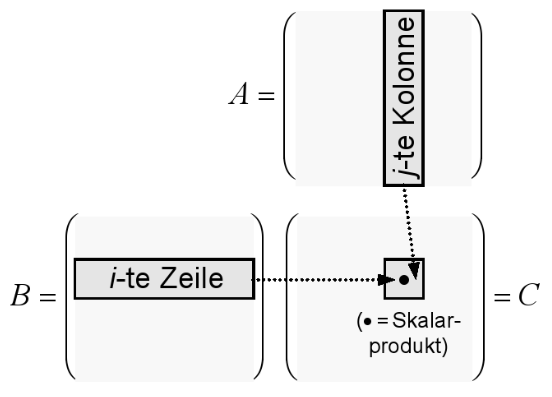
\includegraphics[width=5cm]{./bilder/matrix.png}
        \end{minipage}
		
	\subsection{Einige W-Matrizen}
		\begin{tabular}{l l l l}
        N = 2 & N = 3 & N = 4 & N = 6\\
		$\begin{bmatrix}
		1 & 1\\
		1 & -1\\              
		\end{bmatrix}$ &
		$\begin{bmatrix}
		1 & 1 & 1\\
		1 & -\frac{1}{2}+j\frac{\sqrt{3}}{2} & -\frac{1}{2}-j\frac{\sqrt{3}}{2}\\
		1 & -\frac{1}{2}-j\frac{\sqrt{3}}{2} & -\frac{1}{2}+j\frac{\sqrt{3}}{2}\\
		\end{bmatrix}$ &
		$\begin{bmatrix}
		1 & 1 & 1 & 1 \\
		1 & j & -1 & -j\\
		1 & -1 & 1 & -1\\
		1 & -j & -1 & j\\                   
		\end{bmatrix}$ &
		$\begin{bmatrix}
		1 & 1 & 1 & 1 & 1 & 1\\
		1 & \frac{1}{2}+j\frac{\sqrt{3}}{2} & -\frac{1}{2}+j\frac{\sqrt{3}}{2} & -1
		& -\frac{1}{2}-j\frac{\sqrt{3}}{2} & \frac{1}{2}-j\frac{\sqrt{3}}{2}\\
		1 & -\frac{1}{2}+j\frac{\sqrt{3}}{2} & -\frac{1}{2}-j\frac{\sqrt{3}}{2} & 1
		& -\frac{1}{2}+j\frac{\sqrt{3}}{2} & -\frac{1}{2}-j\frac{\sqrt{3}}{2}\\
		1 & -1 & 1 & -1 & 1 & -1\\
		1 & -\frac{1}{2}-j\frac{\sqrt{3}}{2} & -\frac{1}{2}+j\frac{\sqrt{3}}{2} & 1
		& -\frac{1}{2}-j\frac{\sqrt{3}}{2} & -\frac{1}{2}+j\frac{\sqrt{3}}{2}\\ 
		1 & \frac{1}{2}-j\frac{\sqrt{3}}{2} & -\frac{1}{2}-j\frac{\sqrt{3}}{2} & -1
		& -\frac{1}{2}+j\frac{\sqrt{3}}{2} & \frac{1}{2}+j\frac{\sqrt{3}}{2}\\ 
		\end{bmatrix}$
		\end{tabular}

		\begin{tabular}{l }
        N = 8\\
 		$\begin{bmatrix}
		1 & 1 & 1 & 1 & 1 & 1 & 1 & 1\\ 
		1 & \frac{\sqrt{2}}{2}+\frac{\sqrt{2}}{2}j & j &
		-\frac{\sqrt{2}}{2}+\frac{\sqrt{2}}{2}j & -1 & 
		-\frac{\sqrt{2}}{2}-\frac{\sqrt{2}}{2}j & -j & 
		\frac{\sqrt{2}}{2}-\frac{\sqrt{2}}{2}j\\
		1 & j & -1 & -j & 1 & j & -1 & -j\\
		1 &	-\frac{\sqrt{2}}{2}+\frac{\sqrt{2}}{2}j & -j & 
		\frac{\sqrt{2}}{2}+\frac{\sqrt{2}}{2}j & -1 & 
		\frac{\sqrt{2}}{2}-\frac{\sqrt{2}}{2}j & j &
		-\frac{\sqrt{2}}{2}-\frac{\sqrt{2}}{2}j\\
		1 & -1 & 1 & -1 & 1 & -1 & 1 & -1\\
		1 &	-\frac{\sqrt{2}}{2}-\frac{\sqrt{2}}{2}j & j &
		\frac{\sqrt{2}}{2}-\frac{\sqrt{2}}{2}j & -1 &
		\frac{\sqrt{2}}{2}+\frac{\sqrt{2}}{2}j & -j &
		-\frac{\sqrt{2}}{2}+\frac{\sqrt{2}}{2}j\\
		1 & -j & -1 & j & 1 & -j & -1 & j\\
		1 &	\frac{\sqrt{2}}{2}-\frac{\sqrt{2}}{2}j & -j & 
		-\frac{\sqrt{2}}{2}-\frac{\sqrt{2}}{2}j & -1 &
		-\frac{\sqrt{2}}{2}+\frac{\sqrt{2}}{2}j & j &
		\frac{\sqrt{2}}{2}+\frac{\sqrt{2}}{2}j
		\end{bmatrix}$
		\end{tabular}


	
	
	
	
		%\newpage
		
		%Funktionen
		\section{Funktionen}
	\subsection{Impulsfunktion - Dirac Delta Funktion}
		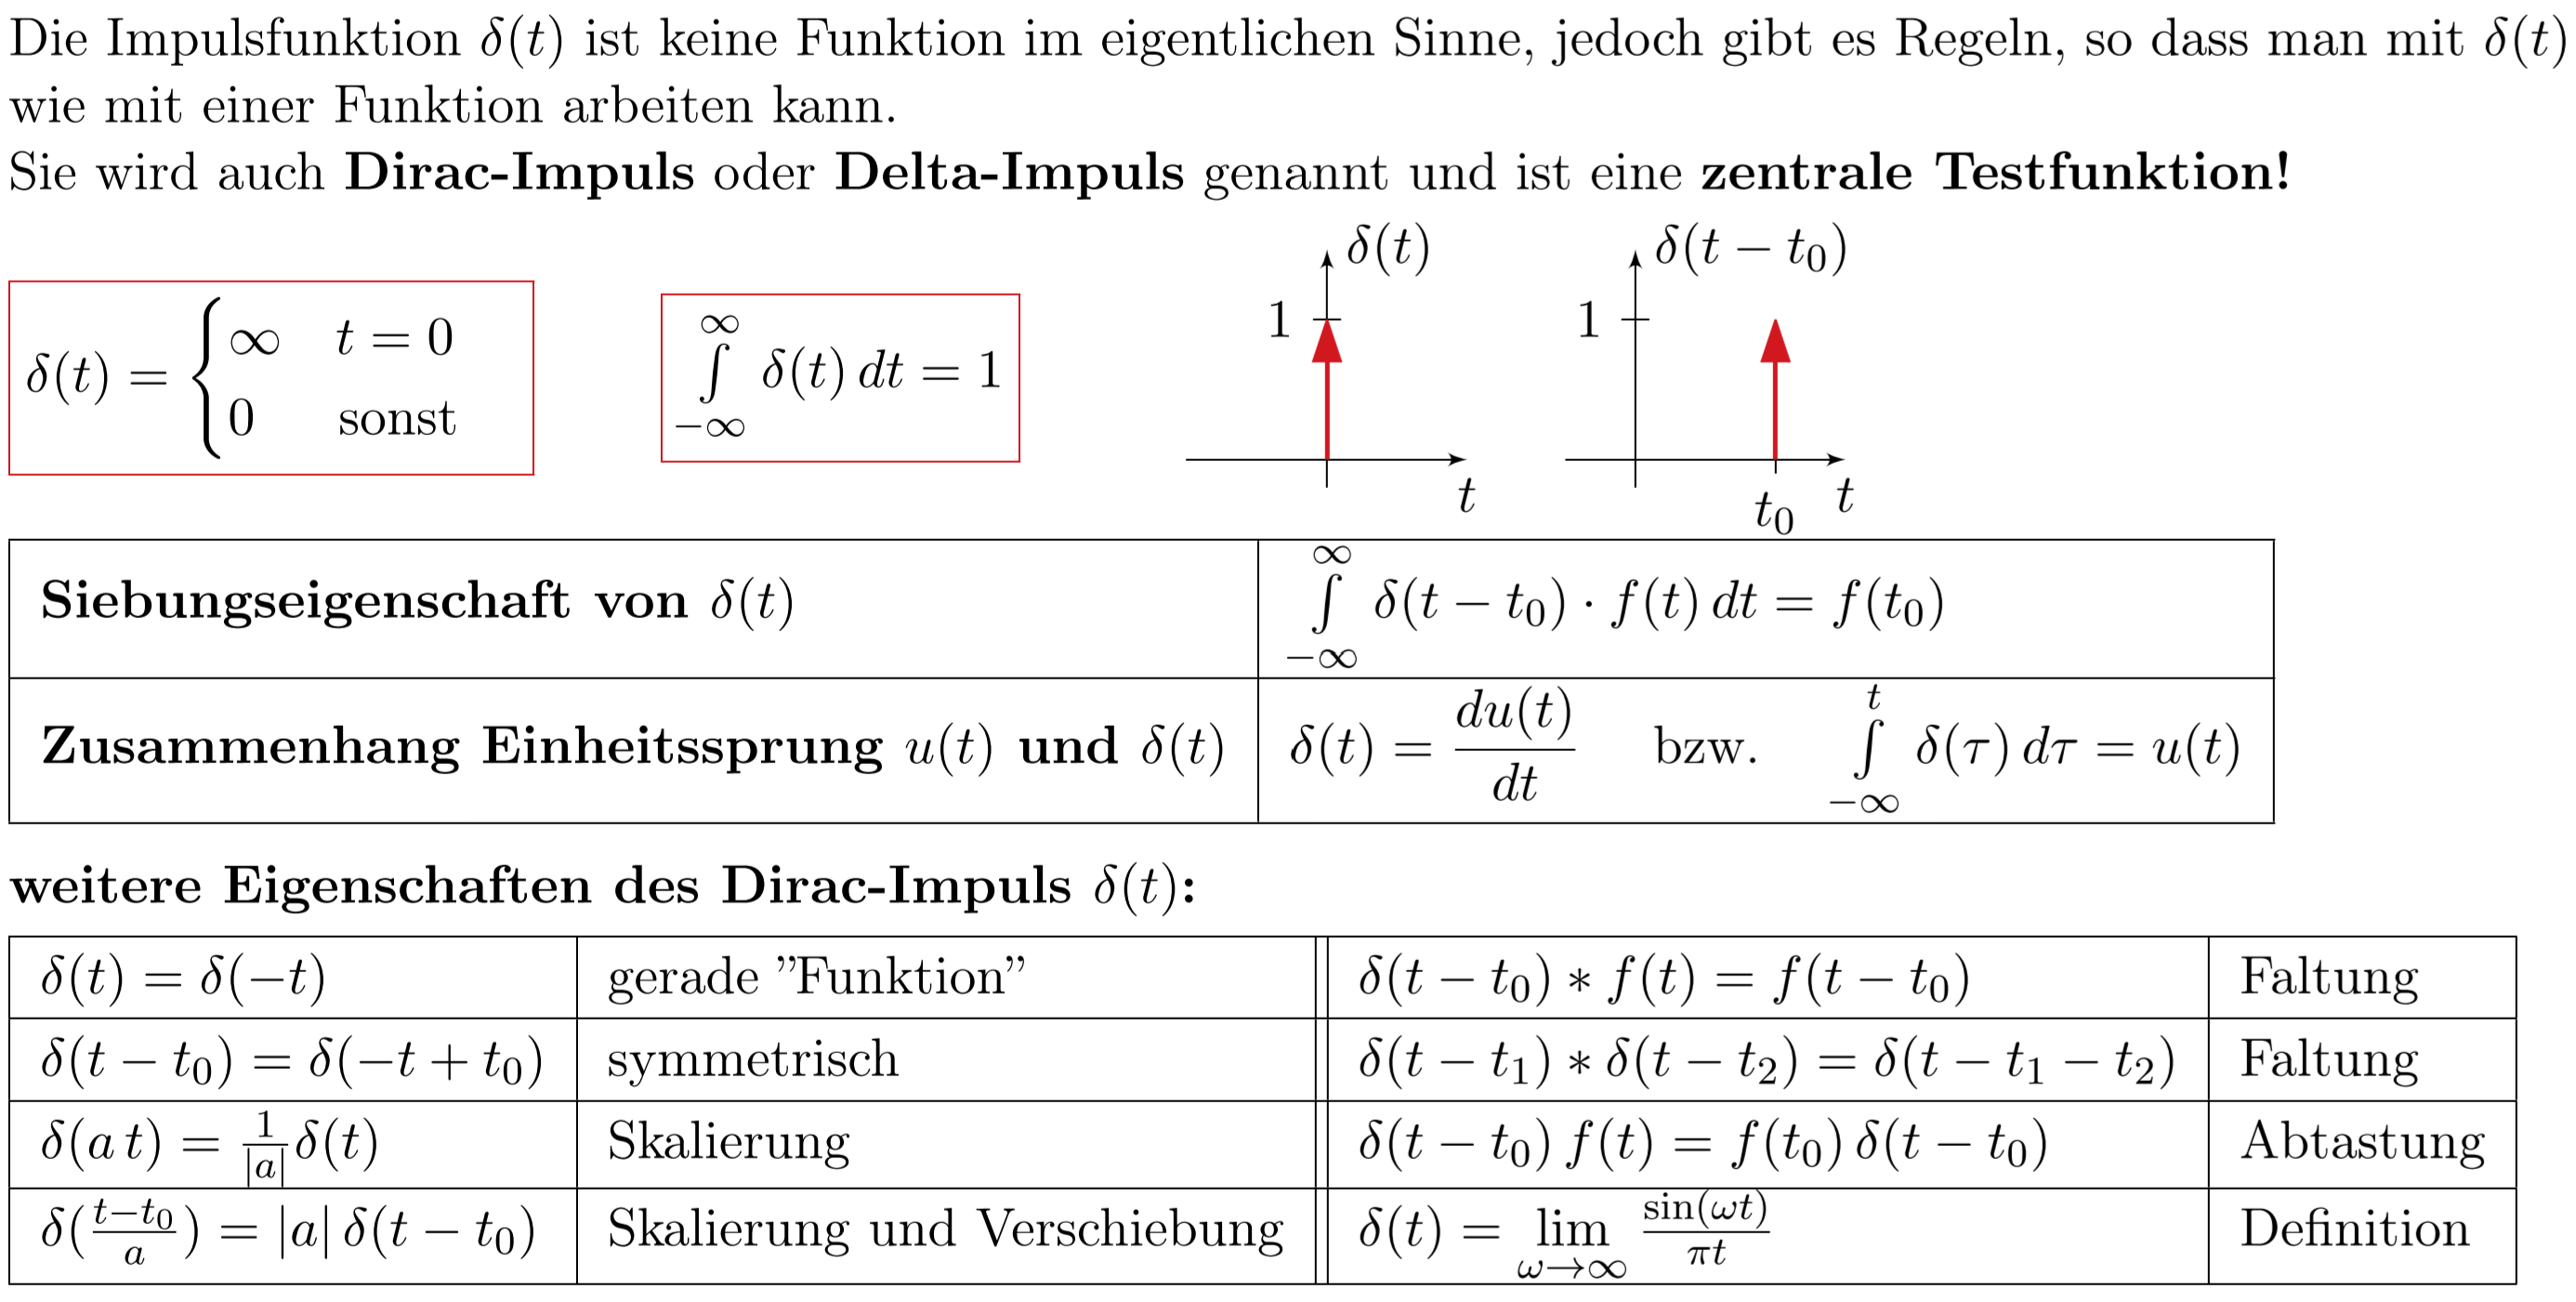
\includegraphics[width=0.8\textwidth]{./bilder/funktionen/impulsF.png}\\
        
        Bei einer Faltung mit einer $\delta\left(t\right)$ Funktion
        gilt: $f\left(t\right) \ast \delta\left(t\right) = f\left(t\right)$
	
	\subsubsection{Fouriertransformierte $\delta(t)$}
		$\delta(t) \; \laplace \; 1(\omega)$ \qquad
		$\delta(t-t_0) \; \laplace \; e^{-j\omega t_0}$ \qquad
		$1(t) \; \laplace \; 2\pi \delta(\omega)$



	\subsection{$\sigma$-Funktion, Schrittfunktion, unit-step}
		\begin{minipage}{0.2\textwidth}
			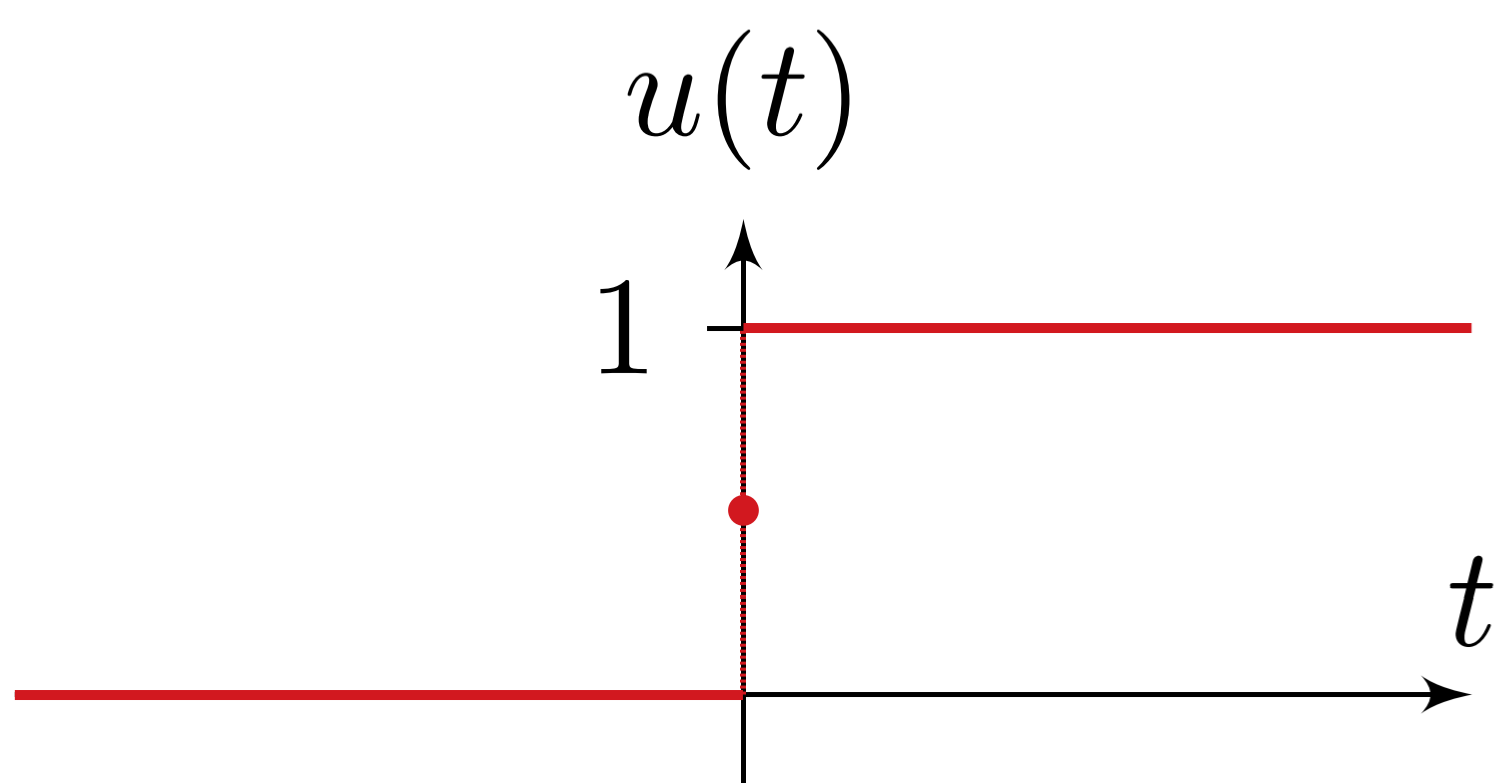
\includegraphics[width=\textwidth]{./bilder/funktionen/sprungF.png}
		\end{minipage}
		\qquad
		\begin{minipage}{0.45\textwidth}
			$u(t) = \sigma(t) =	\begin{cases}
			0 & \text{f\"ur } t < 0 \\
			\frac{1}{2} \text{(praxis)}  \text{ oder undef. (math.)} & \text{f\"ur } t = 0 \\
			1 & \text{f\"ur } t > 0
			\end{cases}$
		\end{minipage}
		\qquad
		\begin{minipage}{0.25\textwidth}						
			$\sigma(t) \; \laplace \; \frac{1}{j\omega} + \pi\delta(\omega) = \Sigma(\omega)$ \\
			\\
			$\frac{du(t)}{dt}=\delta(t)$\\
		\end{minipage}
	
	
	\subsection{Signumfunktion}
		\begin{minipage}{0.2\textwidth}
			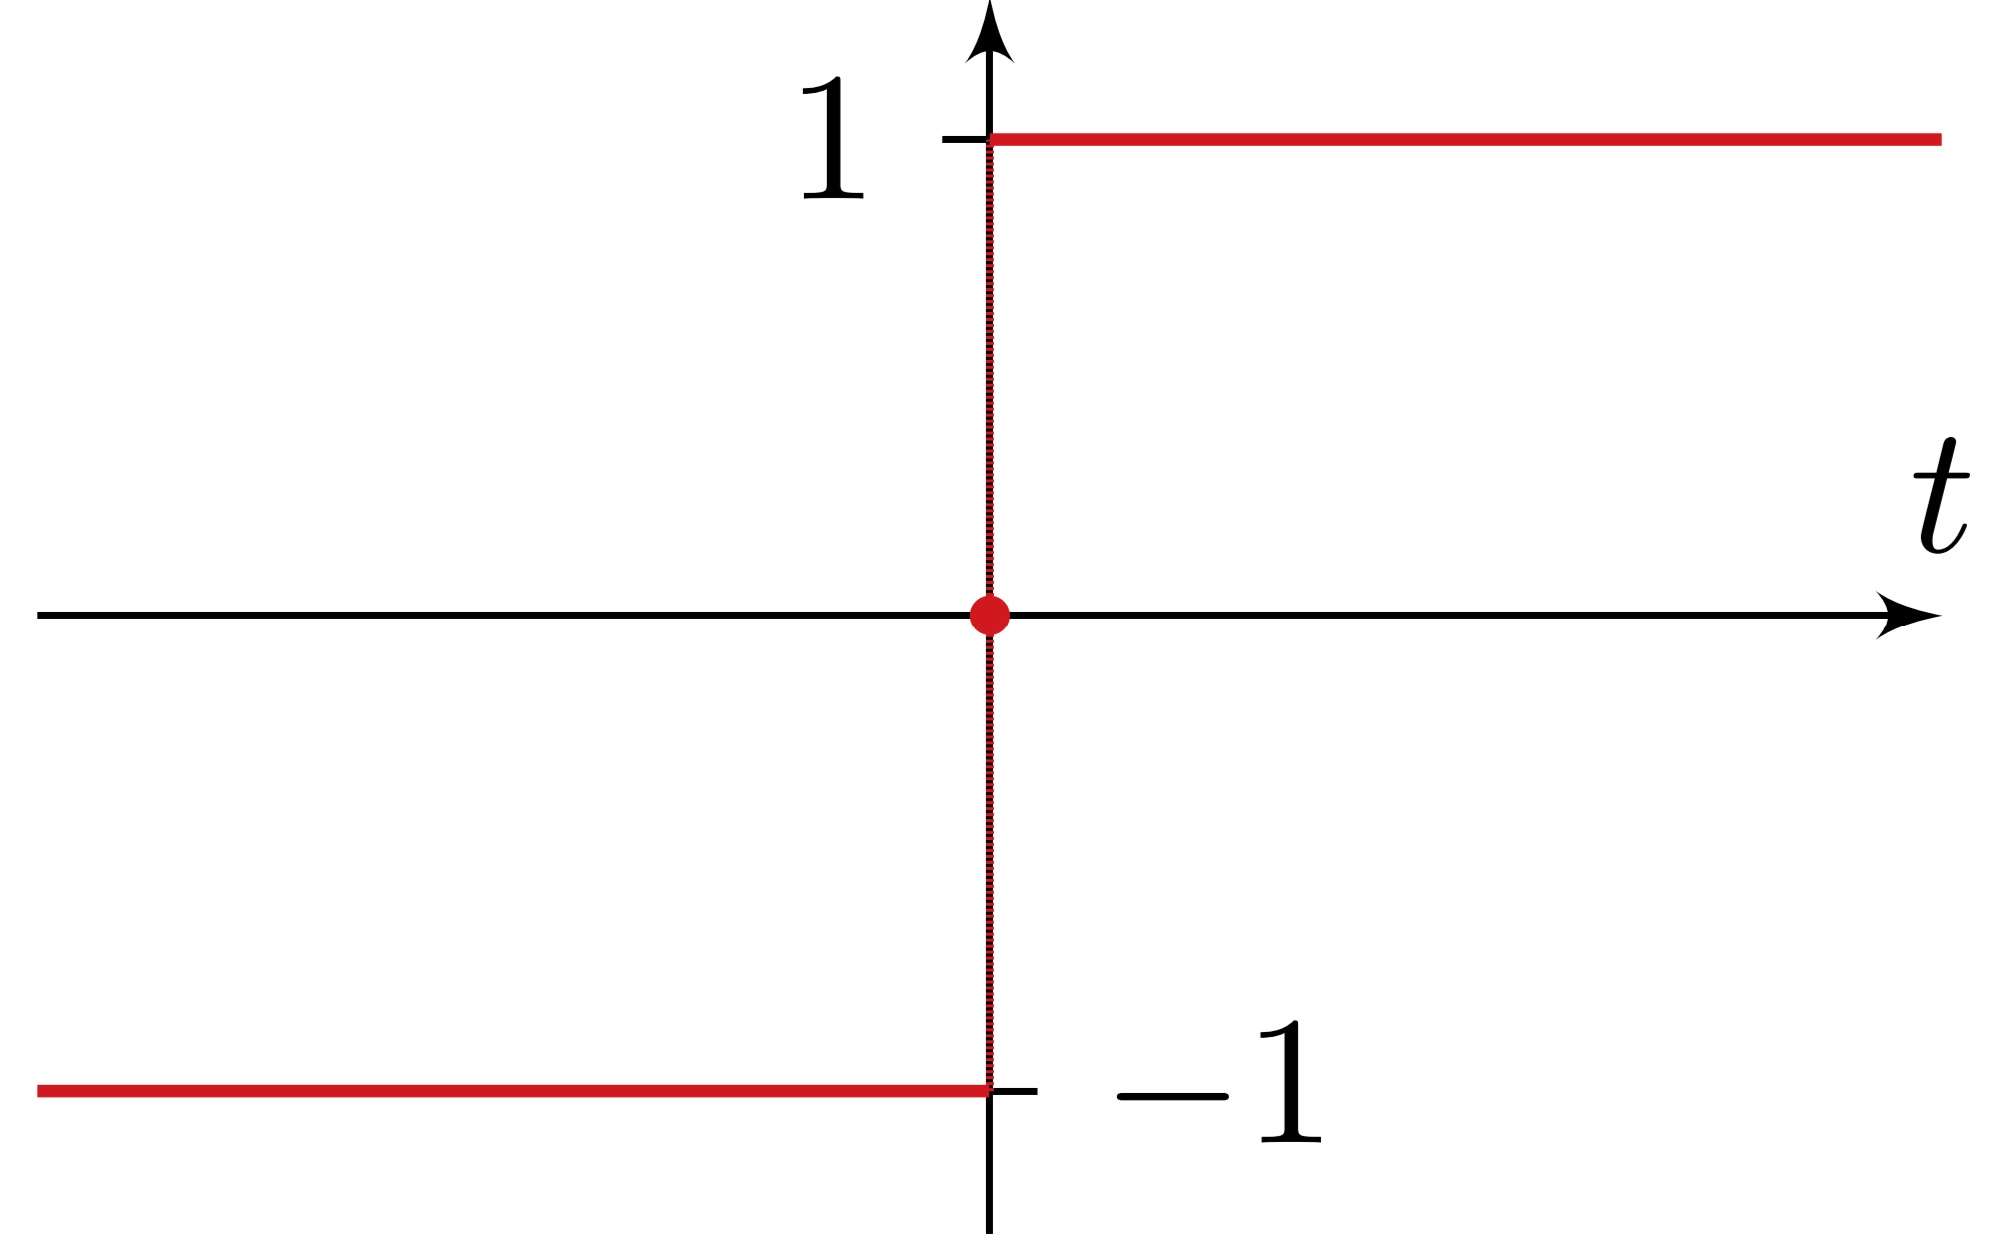
\includegraphics[width=\textwidth]{./bilder/funktionen/signF.png}
		\end{minipage}
		\qquad
		\begin{minipage}{0.45\textwidth}
			$sgn(t) = \begin{cases} 1 & \text{falls }t > 0 \\ -1 & \text{falls }t < 0 \end{cases}$
		\end{minipage}
		\qquad
		\begin{minipage}{0.25\textwidth}
            \begin{math}
                \begin{aligned}
                   sgn(t) \; &\laplace \; \frac{2}{j\omega}\\
                   \frac{1}{\pi t} \; &\laplace \; -j \cdot sgn(\omega)
                \end{aligned}
            \end{math}						
		\end{minipage}		

		
	\subsection{Rechteckimpuls}
		\begin{minipage}{0.2\textwidth}
			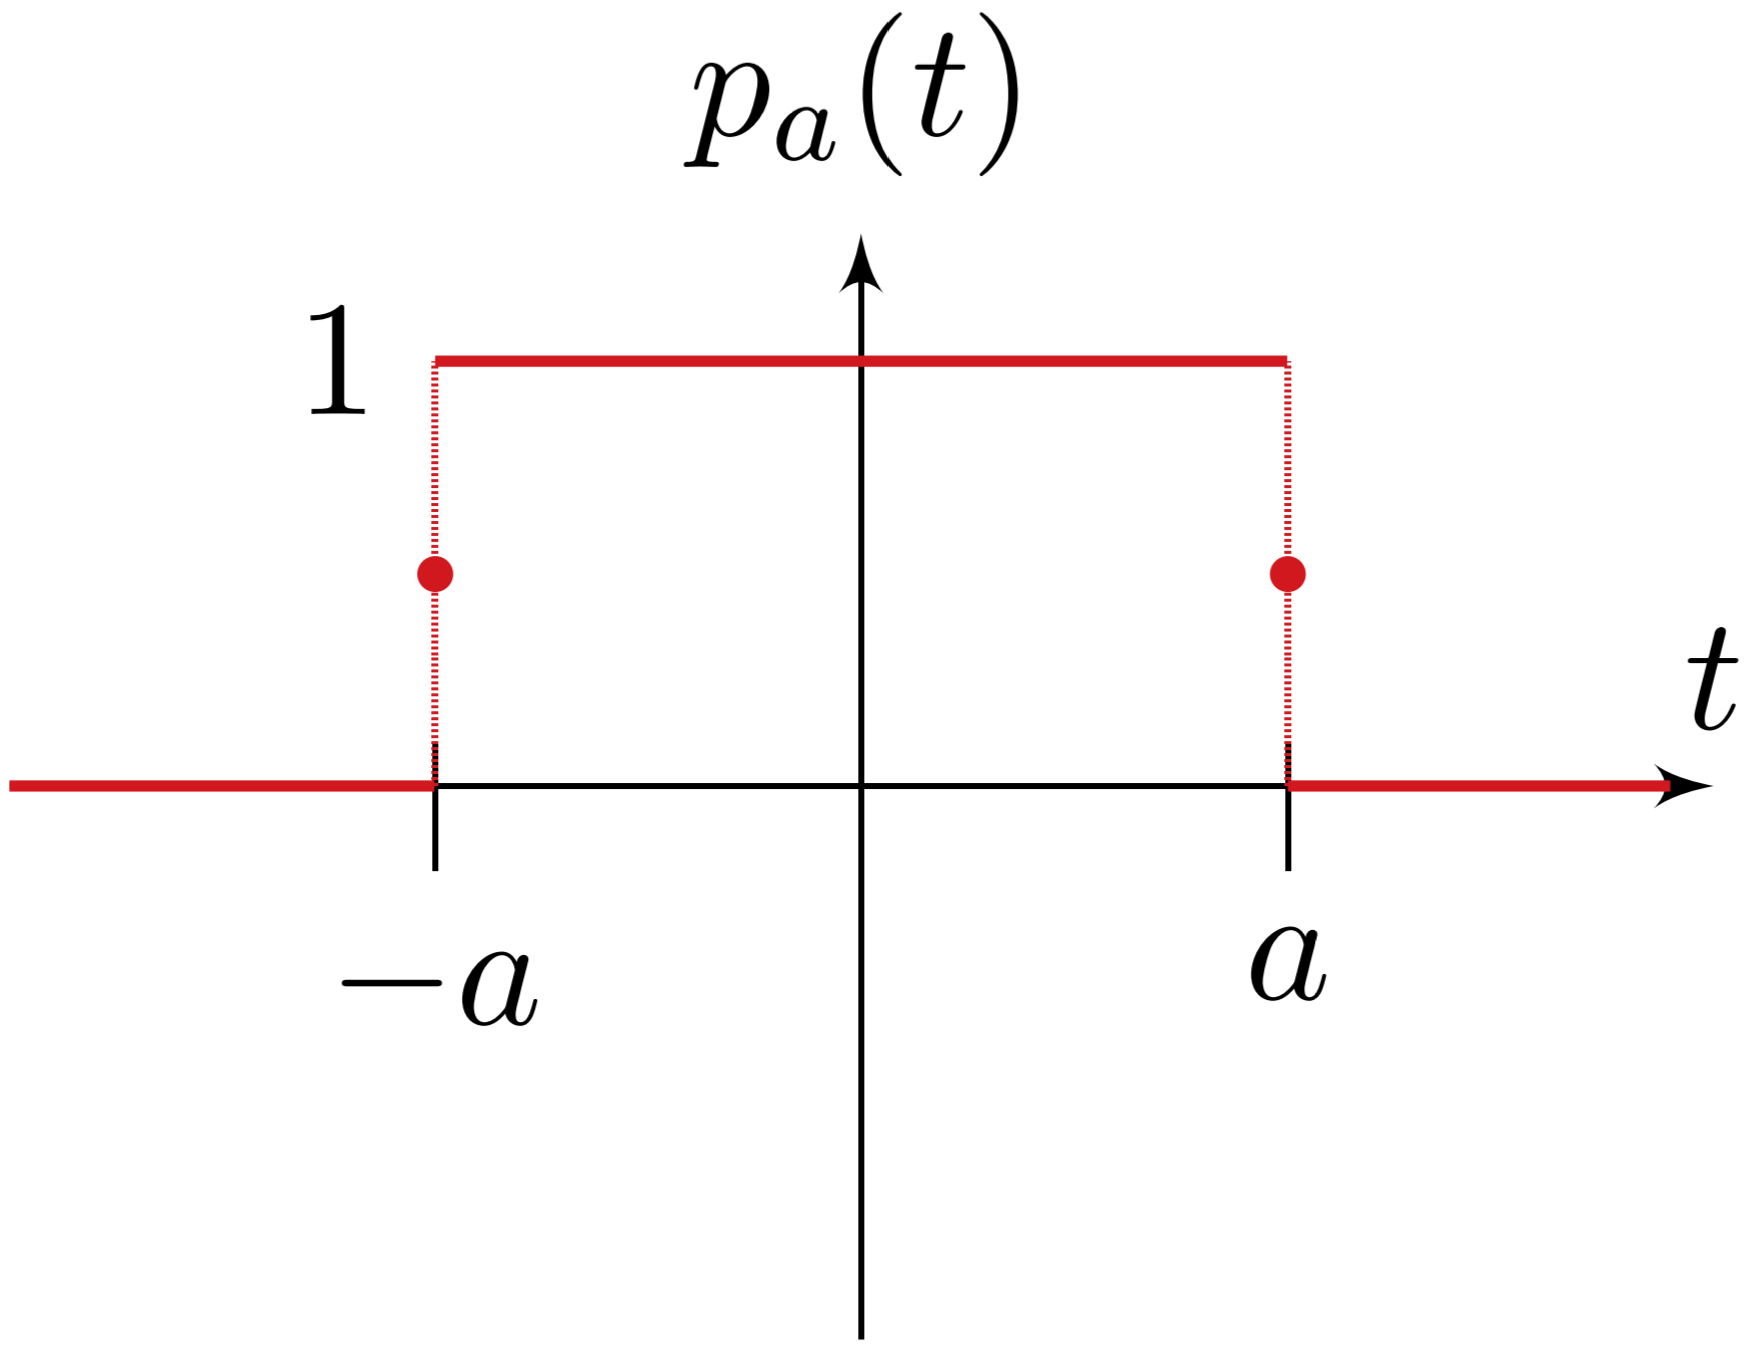
\includegraphics[width=\textwidth]{./bilder/funktionen/rechteckF.png}
		\end{minipage}
		\qquad
		\begin{minipage}{0.45\textwidth}
			$p_{a}(t)=\begin{cases}
							1 & |t|<a \\ 
							\frac{1}{2} & |t|=a \\ 
							0 & |t|>a
						\end{cases}$
		\end{minipage}
		\qquad
		\begin{minipage}{0.25\textwidth}						
			%
		\end{minipage}
	
	\subsection{Rampenfunktion}
		\begin{minipage}{0.2\textwidth}
			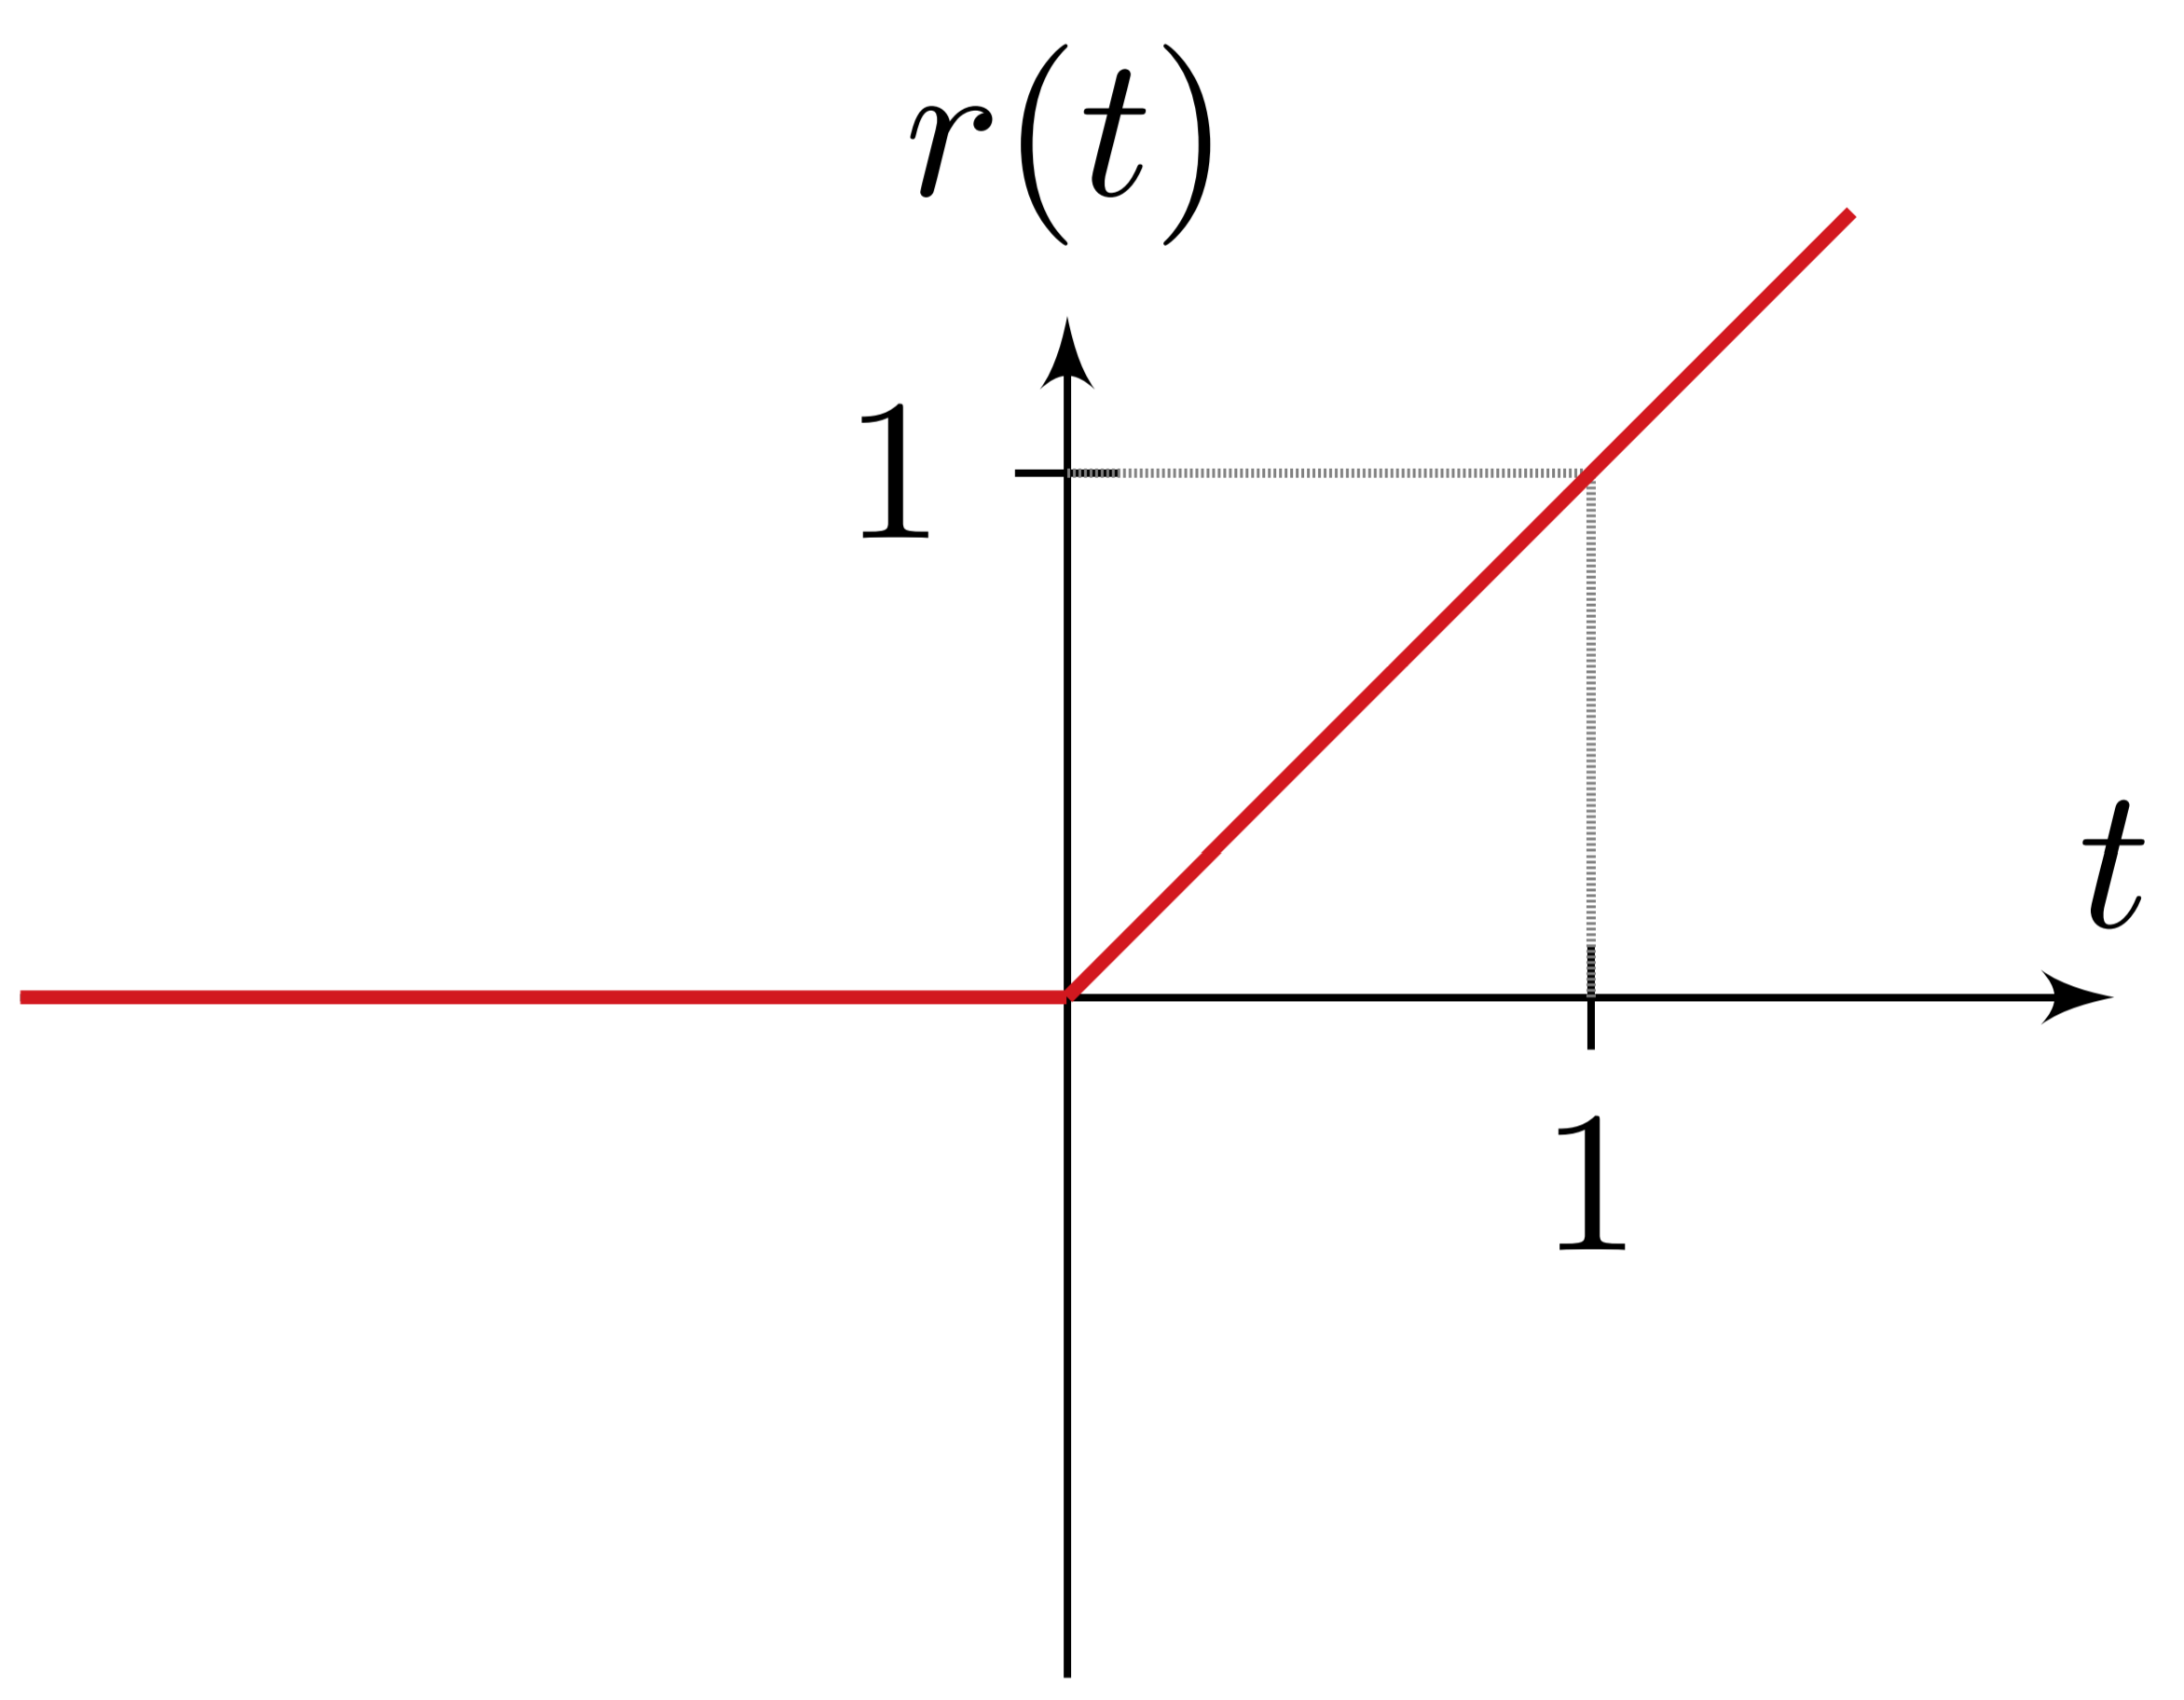
\includegraphics[width=\textwidth]{./bilder/funktionen/rampenF.png}
		\end{minipage}
		\qquad
		\begin{minipage}{0.45\textwidth}
			$r(t)=\begin{cases}
						{0} & {t \leq 0} \\ 
						{t} & {t>0}
					\end{cases}$
		\end{minipage}
		\qquad
		\begin{minipage}{0.25\textwidth}						
			%
		\end{minipage}		
		
	\subsection{Dreieckimpuls}
		\begin{minipage}{0.2\textwidth}
			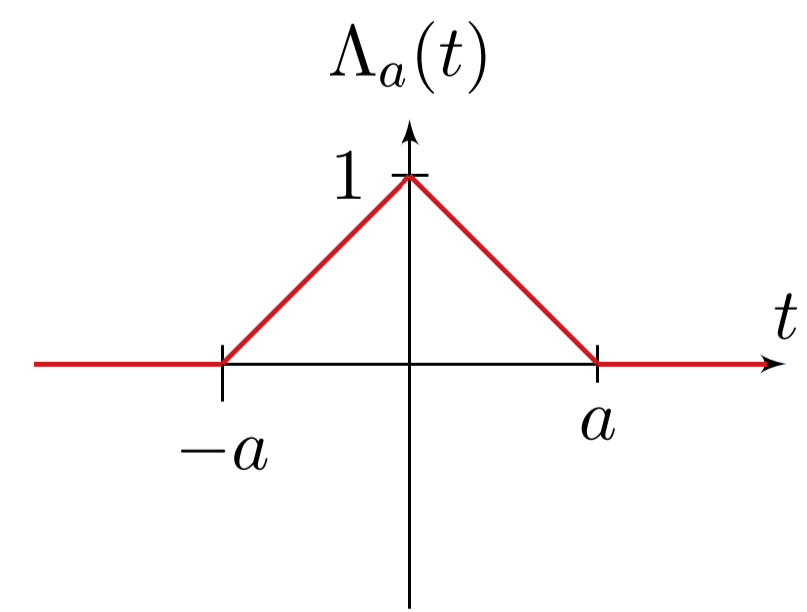
\includegraphics[width=\textwidth]{./bilder/funktionen/dreieckF.png}
		\end{minipage}
		\qquad
		\begin{minipage}{0.45\textwidth}
			$\Lambda_{a}(t)=\begin{cases}{1-\frac{|t|}{a}} & {t<a} \\ {0} & {|t| \geq a}\end{cases}$
		\end{minipage}
		\qquad
		\begin{minipage}{0.25\textwidth}						
			%
		\end{minipage}
	
	
	\subsection{Sinc-Funktion}
				\begin{minipage}{0.2\textwidth}
			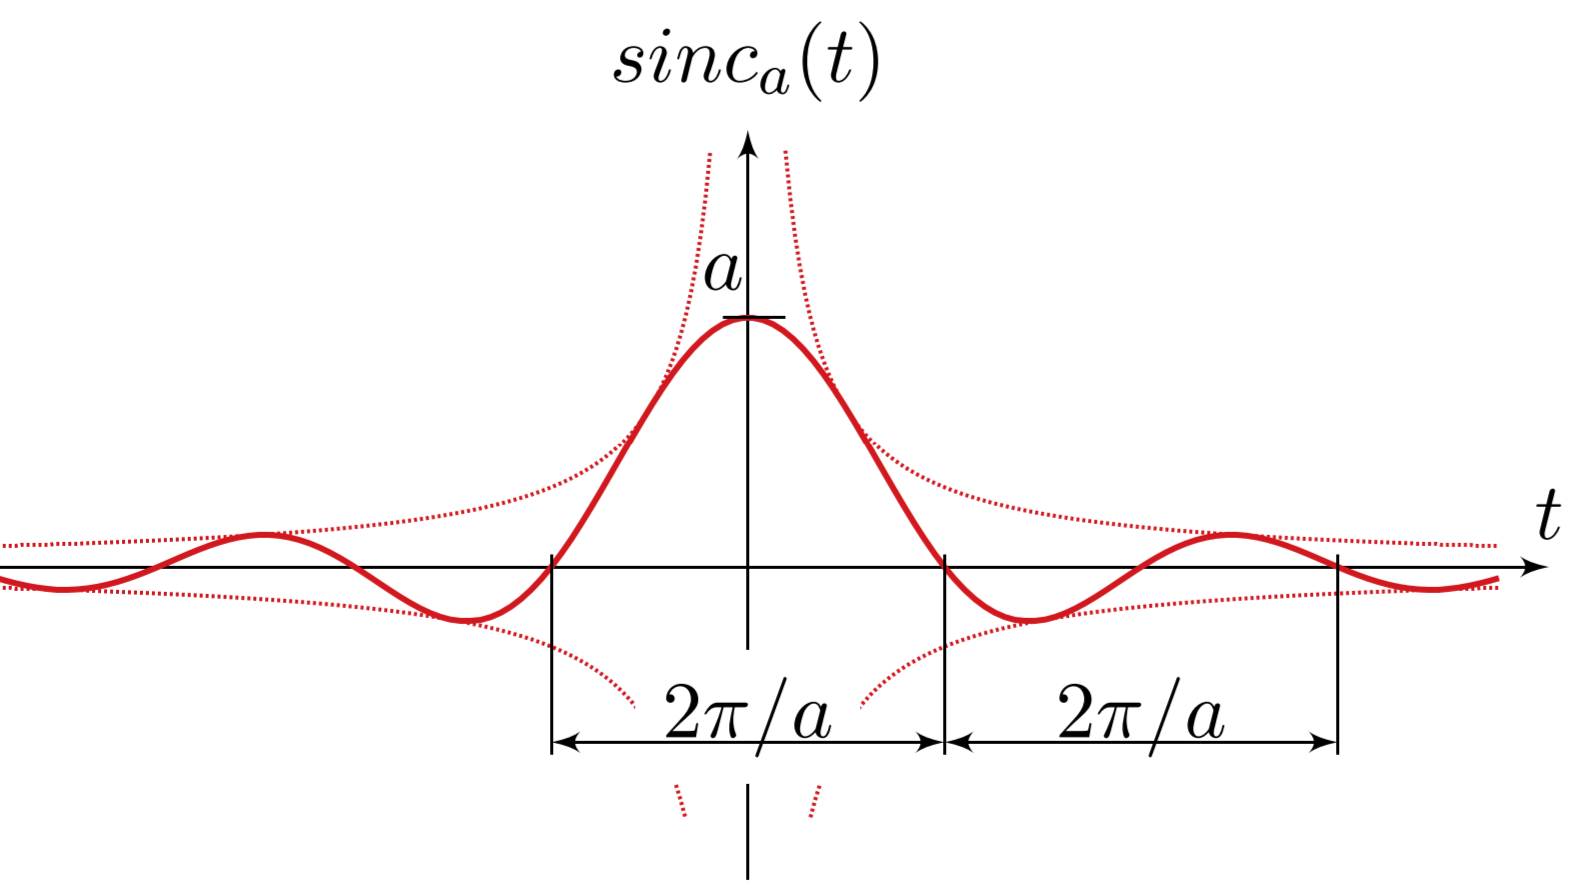
\includegraphics[width=\textwidth]{./bilder/funktionen/sincF.png}
		\end{minipage}
		\qquad
		\begin{minipage}{0.45\textwidth}
			\begin{math}
				\begin{aligned}
					\operatorname{sinc}_{a}(t) &= \frac{\sin (a t)}{t} \\
					\operatorname{sinc}(a t) &= \frac{\sin (a t)}{a t}
				 \end{aligned}
			 \end{math}
		\end{minipage}
		\qquad
		\begin{minipage}{0.25\textwidth}						
			%
		\end{minipage}\\
	
		
		%TODO Berechnungen zu den Funktionen hinzufügen
%		\subsection{Beispiele}
%			\begin{tabular}{l l l}
%				Rechteckimpuls $r_T$ der Breite $2T$ & $r_T \; \laplace \; \frac{2 \cdot \sin(\omega T}{\omega}$ \\
%			\end{tabular}\\
%			\begin{tabular}{p{9cm} p{9cm}}
%				$r_T(t) \; \laplace \; \frac{2}{\omega} \cdot \sin(\omega T) \Rightarrow$ sinc-Funktion &
%				$\int\limits_{-\infty}^{\infty} \frac{\sin(a \omega)}{\omega} d\omega = 
%				\begin{cases} \pi & \text{falls }a > 0 \\ -\pi & \text{falls }a < 0 \end{cases}$
%			\end{tabular}
	
	
	\subsection{Funktionen manipulieren}
		\includegraphics[width=0.8\textwidth]{./bilder/funktionen/SignalManip.png}			%TODO Funktionen mit Transformierten ergänzen
		
	\newpage
		% Fourierreihe
		\section{Fourierreihe}
  	$$\boxed{f(t) = \sum\limits_{k = -\infty}^{\infty} c_k \cdot e^{j k \omega_1
  	t}}= \boxed{\sum\limits_{k = 0}^{\infty} \left(c_k \cdot e^{j k \omega_1
  	t} + \overline{c_k} \cdot e^{-j k \omega_1t}\right)}$$
  	$$\boxed{f(t) = \frac{a_0}{2} + \sum\limits_{k=1}^{\infty} \left[a_k \cos(k
  	\omega_1 t) + b_k \sin(k \omega_1 t)\right]}=\boxed{\frac{A_0}{2} +
  	\sum\limits_{k=1}^{\infty} A_k \cos(k \omega_1 t + \varphi_k)} \quad k\in
  	\mathbb{Z}, \quad \boxed{\omega_1=\frac{2 \pi}{T}=2 \pi f}$$	
	$$\boxed{c_k=\overline{c_{-k}}=\frac{1}{T}\int_0^T{f(t)\cdot
	e^{-jk\omega_1
	t}dt} \; ; \; c_0 = \frac{a_0}{2}} \qquad \boxed{a_0 = \frac{2}{T}\int\limits_0^{T}
	f(t)dt, \quad a_k = \frac{2}{T}\int\limits_0^{T} f(t)\cos(k \omega_1 t) dt, \quad b_k =
	\frac{2}{T}\int\limits_0^{T} f(t)\sin(k \omega_1 t) dt}$$
	$a_0$, $c_0$, $A_0$ sind \textit{Konstanten}, $\omega_1$ ist die
	\textit{Grundkreisfrequenz}, $a_k$ und $b_k$ sind die \textit{reellen
	Koeffizienten}, $c_k$ ist der \textit{komplexe Koeffizient}, $A_k$ ist die
	\textit{Amplitude} und $\varphi_k$ ist die \textit{Phase}.\\
	\fbox{
	\begin{tabular}{p{9cm}p{9cm}}
		$a_k = c_k + \bar{c_k} = 2\Real(c_k) = A_k \cos(\varphi_k)$ &
		$b_k = j(c_k + \bar{c_k}) = -2\Imag(c_k) = -A_k \sin(\varphi_k)$ \\
		$c_k = \frac{a_k-jb_k}{2} = \frac{A_k}{2} e^{j\varphi_k} = \frac{\pi}{T}F(j k \omega)$ &
		$c_{-k} = \overline{c_k} = \frac{a_k+jb_k}{2} = \frac{A_k}{2} e^{-j\varphi_k}$ \\
		$A_k = 2|c_k| = \sqrt{a_k^2+b_k^2}$ & $\varphi_k =  \arg(c_k)$ oder unten $\downarrow$\\
	\end{tabular}}\\

	\textbf{Berechnung von $\varphi_k$ aus $a_k$ und $b_k$}\\
	\begin{tabular}{p{4cm}p{4cm}p{3cm}p{3.5cm}}
		$a_k> 0:$ & $\varphi_k = -\arctan(\frac{b_k}{a_k})$ &
		$a_k<0:$ &	$\varphi_k = -\arctan(\frac{b_k}{a_k}) + \pi$\\
		$a_k = 0 \wedge b_k > 0:$ &	$\varphi_k = -\frac{\pi}{2}$ &
		$a_k = 0 \wedge b_k < 0:$ &	$\varphi_k = \frac{\pi}{2}$\\
		$a_k = 0 \wedge b_k = 0:$ &	$\varphi_k = \text{nicht definiert}$
	\end{tabular}

	\subsection{Symmetrie}
		\begin{tabular}{|p{4.3cm}|p{4.3cm}|p{4.4cm}|p{4.4cm}|}
         	\hline
        	\textbf{gerade Funktion} & \textbf{ungerade Funktion} &
        	\textbf{Halbperiode 1} & \textbf{Halbperiode 2}\\
        	\hline
        	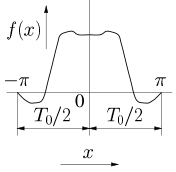
\includegraphics[width=3cm,trim=0 0 0 -5]{./bilder/gerade_funktion.png}&
        	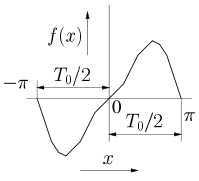
\includegraphics[width=3cm]{./bilder/ungerade_funktion.png}&
 			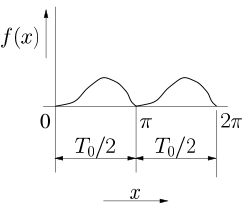
\includegraphics[width=3cm]{./bilder/halbperiode_1.png}&   
			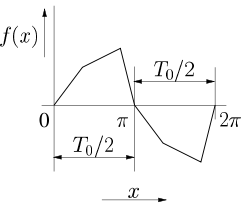
\includegraphics[width=3cm]{./bilder/halbperiode_2.png}\\
			\hline & & & \\			
   			$f(-t)=f(t)$ & $f(-t)=-f(t)$ & $f(t)=f(t+\pi)$ & $f(t)=-f(t+\pi)$\\
   			$b_k=0$ & $a_k=0$ & $a_{2k+1}=0$ & $a_{2k}=0$\\
   			$a_k = \frac{4}{T} \int\limits_0^{\frac{T}{2}} f(t) \cdot \cos(k \omega_1
   			t) dt$ &
   			$b_k =  \frac{4}{T} \int\limits_0^{\frac{T}{2}} f(t) \cdot
			\sin(k \omega_1 t) dt$ &
			$b_{2k+1}=0$ & $b_{2k}=0$\\
			\hline
      	\end{tabular}

	\subsection{Rechtecksignale}
	$$a_k=\frac{2}{T}\int\limits_{-t_1/2}^{t_1/2}A\cos\left(\frac{2\pi k}{T}t\right)dt=
	\left .\frac{2AT}{2\pi T k}\sin \left(\frac{2\pi k}{T}t\right)\right |_{-t_1/2}^{t_1/2}=
	\frac{2A}{\pi k}\sin\left(\frac{\pi t_1}{T}k\right)$$
	
	F"ur Verh"altnisse $\frac{T}{ggT(t_1,T)}=n\in\mathbb{N}$ verschwinden die
	$n.$ Harmonische und deren Vielfache.\\
	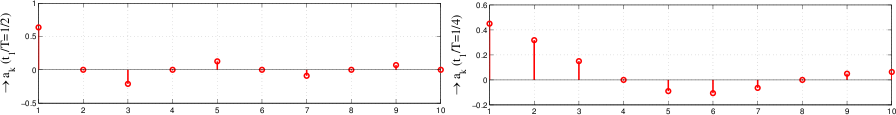
\includegraphics[width=19cm]{./bilder/fourierreihe-rechteck.png}
	\newpage	
	
		% Fourier-Integral / Fourier-Transformation
		\section{Fourier-Transformation}
\begin{tabular}{|p{6cm} l|} \hline
	\textbf{Fouriertransformierte:} &
	$F(j\omega) = \int\limits_{-\infty}^{\infty} f(t)e^{-j\omega t}dt$ \\
	\textbf{Rücktransformierte:} &
	$f(t) = \frac{1}{2\pi}\int\limits_{-\infty}^{\infty}F(j\omega)e^{j\omega t}d\omega$ \\ \hline
\end{tabular} \\
\begin{tabular}{p{6cm} l}
Dies ergibt das \textbf{Korespondenzpaar:}	& $f(t) \laplace F(\omega)$ \\
											 & $F(t) \laplace 2\pi \cdot f(-\omega)$ \\
\end{tabular} \\
\begin{tabular}{p{6cm} l}
$F(\omega) = R(\omega) -jX(\omega)$ wobei &
$R(\omega) = \int\limits_{-\infty}^\infty f(t)\cdot \cos(\omega t)\,dt \quad \text{und} \quad X(\omega) =
\int\limits_{-\infty}^\infty f(t)\cdot \sin(\omega t)\,dt$ \\
 & $f(t)$ gerade: $X(\omega)$ verschwindet, f(t) ungerade: $R(\omega)$ verschwindet \\
\end{tabular} \\

Jede reelle $f(t)$ lässt sich aus Summe einer geraden und einer ungeraden Funktion beschreiben:\\
\begin{tabular}{lll}
$f(t) = f_e(t) + f_o(t)$ mit & $f_e(t) = \frac{1}{2}[f(t) + f(-t)]$ & $f_o(t) = \frac{1}{2}[f(t) - f(-t)]$ \\

Also: & $R(\omega) = 2 \int\limits_0^\infty f_e(t) \cos(\omega t)\,dt$ & $X(\omega) = 2 \int\limits_0^\infty
f_o(t) \sin(\omega t)\,dt$ \\

Und: & $f_e(t) = \frac{1}{\pi}\int\limits_0^\infty R(\omega)\cos(\omega t)\,d\omega$ & 
$f_o(t) = \frac{1}{\pi}\int\limits_0^\infty X(\omega)\sin(\omega t)\,d\omega$ \\
\end{tabular}

Bei \textbf{kausalen} Funktionen gilt:\\
$f_e(t) = f_o(t) = \frac{1}{2}f(t) \quad \quad \quad
f(t) = \frac{2}{\pi}\int\limits_0^\infty R(\omega) \cos(\omega t)\,dt = \frac{2}{\pi}\int\limits_0^\infty X(\omega)
\sin(\omega t)\,dt$

\begin{tabular}{|l|l|l|}
\hline
Spektraldichte / Spektraldarstellung	& $F(\omega)$ 		& KEINE absoluten Werte für Amplitude \& Phase \\
\hline
Amplitudendichte 						& $|F(\omega)| $		& f reell $\rightarrow$
$|F(\omega)|$ symetrisch zur Ordinatenachse
\\
\hline
Phasendichte							& $arg(F(\omega))$	& f reell $\rightarrow$ $arg(F(\omega))$ punktsymetrisch zum Ursprung \\
\hline
Kosinusamplitudendichte					& $R(\omega)$		& f reell $\rightarrow$ $R(\omega)$ gerade \\
\hline
Sinusamplitudendichte					& $X(\omega)$ 		& f reell $\rightarrow$ $X(\omega)$ ungerade \\
\hline
Dämpfung / Amplitudengang				& $A(\omega) = |H(\omega)|$ & $= \sqrt{H(\omega)\cdot \overline{H(\omega)}}$  \\
\hline
Phasenverschiebung						& $\Phi(\omega) = arg(H(\omega))$ & $= \arctan(\frac{Im(H(\omega))}{Re(H(\omega))})$ \\
\hline
\end{tabular}

\subsection{Symmetrie}
	Es gelten die gleichen Symmetrien wie bei der Fourierreihe.

\subsection{Hilbert-Transformation}
Das folgende Paar heisst \textit{Hilbert-Transformationspaar} und ermöglicht die Berechnung von Real- und Imaginärteil
einer Fouriertransformation auseinander. \\ 

\begin{tabular}{|l|} \hline
$\Re(\omega) = \frac{1}{\pi} \cdot \int\limits_{-\infty}^{\infty} \frac{\Im(u)}{\omega-u}du$ \\
$\Im(\omega) = -\frac{1}{\pi} \cdot \int\limits_{-\infty}^{\infty} \frac{\Re(u)}{\omega-u}du$ \\ \hline
\end{tabular} \\

Allgemein ist die Hilbert-Transformation $\mathcal{H}$ folgendermassen definiert: \\
$\mathcal{H}(f(t)) := \frac{1}{\pi} \cdot \int\limits_{-\infty}^{\infty} \frac{f(u)}{t-u}du$ \\

\subsection{Eigenschaften}
		\begin{tabular}{|p{8cm}|p{8cm}|}
        	\hline
        	Linearität & 
        	$\alpha\cdot f(t) + \beta\cdot g(t) \laplace \alpha\cdot F(j\omega) +
        	\beta\cdot G(j\omega)$\\
        	\hline
			Zeitumkehrung (Spiegelung an der Y-Achse)&
			$f(-t) \laplace F(-j\omega) = F^*(jw)$ \\
			\hline        	
  			"Ahnlichkeit / Zeitskalierung &
  			$f(\alpha t) \laplace \frac{1}{|\alpha|}F \left (j\frac{\omega}{\alpha} \right)
  			\quad\alpha \in\mathbb{R}\setminus \{0\}$\\
  			\hline
  			Verschiebung im	Zeitbereich &
  			$f(t\pm t_0) \laplace F(j\omega)e^{\pm j\omega t_0}$\\
  			\hline
			Verschiebung im Frequenzbereich &
			$f(t)e^{\pm j\omega_0 t} \laplace F(j(\omega\mp\omega_0))$\\
			\hline
			Ableitung im Zeitbereich &
			$\frac{\partial^n f(t)}{\partial t^n} \laplace (j\omega)^n F(j\omega)$\\
			\hline
			Integration im Zeitbereich &
			$\int\limits_{-\infty}^{t}f(\tau)d\tau \laplace
			\frac{F(j\omega)}{j\omega}+F(0)\pi\delta(\omega)$\\
			\hline				
			Ableitung im Frequenzbereich &
			$t^n f(t) \laplace j^n \frac{\partial F(j\omega)}{\partial \omega^n}$\\
			\hline		
			Faltung im Zeitbereich &
			$f(t) \ast g(t) = \int\limits_{-\infty}^{\infty} f(\tau)g(t-\tau)d\tau \laplace
			F(j\omega) \cdot G(j\omega)$\\
			\hline
			Faltung im Frequenzbereich &
			$f(t) \cdot g(t) \laplace \frac{1}{2\pi}F(j\omega) \ast G(j\omega)$\\
			\hline
			Vertauschungssatz (Dualität) &
			$f(t) \laplace F(j\omega)\nonumber$ \\
 			& $F(t) \laplace 2\pi \cdot f(-j\omega)$\\
 			\hline
 			Modulation &
 			$\cos(\alpha t) \cdot f(t)  \laplace  \frac{1}{2}\cdot
 			\left[F(j(\omega-\alpha)) + F(j(\omega+\alpha))\right ]$\\
 			& $\sin(\alpha t) \cdot f(t) \laplace \frac{1}{2j}\cdot \left[
 			F(j(\omega-\alpha)) - F(j(\omega+\alpha))\right ]$\\
 			\hline
        	Parseval's Theorem &
 			$\int\limits_{-\infty}^{\infty}f(t)g^{\ast}(t)dt = \frac{1}{2\pi}
  			\int\limits_{-\infty}^{\infty}F(j\omega)G^{\ast}(j\omega)d\omega$\\
  			\hline
  			Bessel's Theorem &
  			$\int\limits_{-\infty}^{\infty}|f(t)|^2 dt = \frac{1}{2\pi}
  			\int\limits_{-\infty}^{\infty}|F(j\omega)|^2 d\omega$\\
  			\hline 			
			Anfangswerte &
			$f(0)=\frac{1}{2\pi}\int\limits_{-\infty}^{\infty}F(j\omega)d\omega
			\hspace*{1cm} F(0)=\int\limits_{-\infty}^{\infty}f(t)dt$\\
			\hline
			$\infty$ lange Folge von $\delta$-Impulsen &
			$\sum_{n=-\infty}^{\infty} \delta(t-n\cdot t_0) \laplace
			\sum_{n=-\infty}^{\infty} \frac{2\pi}{t_0}\delta(\omega-n\cdot
			\frac{2\pi}{t_0})$\\
			\hline
        \end{tabular}
        
\subsection{Beispiele}
\begin{tabular}{l l}
Rechteckimpuls $r_T$ der Breite $2T$ & $r_T \laplace \frac{2 \cdot \sin(\omega T}{\omega}$ \\
Signum-Funktion & $\frac{1}{\pi \cdot t} \laplace -j \cdot sgn(\omega)$ \\
				& $sgn(t) \laplace \frac{2}{j\omega}$ \\
\end{tabular}

		\subsection{Hilbertransformation \skript{53}} 
		Das folgende Paar heisst \textit{Hilbert-Transformationspaar} und ermöglicht die Berechnung von Real- und Imaginärteil
		einer Fouriertransformation auseinander. \\ 
		
		\begin{tabular}{|l|} \hline
			$\Re(\omega) = \frac{1}{\pi} \cdot \int\limits_{-\infty}^{\infty} \frac{\Im(u)}{\omega-u}du$ \\
			$\Im(\omega) = -\frac{1}{\pi} \cdot \int\limits_{-\infty}^{\infty} \frac{\Re(u)}{\omega-u}du$ \\ \hline
		\end{tabular}
		\hspace{5mm}bzw. für analytische Signale: \hspace{5mm}
		\begin{tabular}{|l|} \hline
			$s_R(t) = - \frac{1}{\pi} \int\limits_{-\infty}^{\infty} \frac{s_I(u)}{t-u} du$ \\
			$s_I(t) = \frac{1}{\pi} \int\limits_{-\infty}^{\infty} \frac{s_R(u)}{t-u} du$ \\ \hline
		\end{tabular} \\
		
		Allgemein ist die Hilbert-Transformation $\mathcal{H}$ folgendermassen definiert: \\
		$\mathcal{H}(f(t)) := \frac{1}{\pi} \cdot \int\limits_{-\infty}^{\infty} \frac{f(u)}{t-u}du$ \\
		Die Hilbert-Transformation eines Signals $s(t)$ ist gegeben durch die Faltung: \\
		$\mathcal{H}(s(t)) = s(t) * \frac{1}{\pi t}$ mit $\frac{1}{\pi t} \: \; \laplace \; \: -j \cdot sgn(\omega)$ \\
		
			\begin{tabular}{| l | l l |}
				\hline
					Fourier-Transformierte: & $F(\omega) = \mathfrak{R}(\omega) + \im \mathfrak{I}(\omega)
					= \frac{1}{\pi \im} \int\limits_{-\infty}^{\infty}\frac{\mathfrak{R}(u) + \im \mathfrak{I}(u)}{\omega - u} du$ & \\
				\hline
					Hilbert-Transformationspaar: & $\mathfrak{R}(\omega) = \frac{1}{\pi} \int\limits_{-\infty}^{\infty} \frac{\mathfrak{I}(u)}{\omega - u} du$ & (Realteil)\\
					& $\mathfrak{I}(\omega) = -\frac{1}{\pi} \int\limits_{-\infty}^{\infty} \frac{\mathfrak{R}(u)}{\omega - u} du$ & (Imaginärteil)\\
				\hline
					Hilbert-Transformation $\mathcal{H}$: & $\mathcal{H}(f(t)) = \frac{1}{\pi} \int\limits_{-\infty}^{\infty} \frac{f(u)}{t-u} du
					= f(t) * \frac{1}{\pi t}$ & \\
				\hline
					Analytisches Signal: & $s_R(t) = - \frac{1}{\pi} \int\limits_{-\infty}^{\infty} \frac{s_I(u)}{t-u} du$ & (Realteil)\\
					& $s_I(t) = \frac{1}{\pi} \int\limits_{-\infty}^{\infty} \frac{s_R(u)}{t-u} du$ & (Imaginärteil)\\
				\hline
			\end{tabular}\\
		
			Die Hilbert-Transformation eines Signals $s(t)$ ist gegeben durch die Faltung $s(t) * \frac{1}{\pi t}$ mit $\frac{1}{\pi t} \; \laplace \; -j \cdot sgn(\omega)$.\\
			Durch die Hilbert-Transformation lässt es sich einfach die Fourier-Transformierte berechnen, wenn der Realteil oder der Imaginärteil gegeben
			ist.
	\newpage
		% Abtasttheoreme, diskrete Frouriertransformation
		%Abtasttheorem und diskrete Fouriertransformation

\section{Abtasttheorem, diskrete Fouriertransformation}
	\begin{minipage}{12cm}
		Abtasten einer Funktion mit idealem Abtaster und Abtastintervall $\Delta t$.\\
		$ \scalebox{1.2}{$f(t) \cdot \delta_{\Delta t}(t) = \sum\limits_{k=-\infty}^{\infty} \Delta t \cdot f(k \Delta t) \cdot \delta(t-k \Delta t) $}$
	\end{minipage}
	\begin{minipage}{6cm}
		\begin{tabular}{|l l l|}
			\hline
				Periodisieren &$\laplace$ & Abtasten\\
				Abtasten & $\laplace$ & Periodisieren\\
			\hline
		\end{tabular}
	\end{minipage}

\subsection{Abtasttheoreme}
	\textbf{Kardinalreihe:}  $\scalebox{1.2}{$S(\omega) = \sum\limits_{k=-\infty}^{\infty} S(k\frac{\pi}{T}) \cdot \frac{\sin(\omega T - k\pi)}{\omega T - k\pi}$
	mit $S(k\frac{\pi}{T}) = 2Tc_k$}$\\

	\textbf{Abtasttheorem f\"ur die Frequenz:}
	F\"ur ein Signal von endlicher Dauer $2T$ ist die Fouriertransformierte durch ihre Abtastwerte an den Stellen $k\frac{\pi}{T}$
	vollst\"andig bestimmt. \\
	
	\textbf{Abtasttheorem von Shannon:}
	Ist ein Signal bandbegrenzt mit Grenzfrequenz $\omega_g$, so l\"asst sich das Signal anhand der Abtastwerte zu den Zeitpunkten
	$k\frac{\pi}{\omega_g}$ vollst\"andig rekonstruieren.
	
	
\subsection{Diskrete Fouriertransformation}
\begin{minipage}{14cm}
	mit $N$ Abtastpunkten\\
	-	Die DFT liefert nur $\frac{N}{2}$ unabh\"angige Koeffizienten, da $\hat{c_k}$ und $\hat{c_{-k}}$ konjugiert komplex sind.\\
	- Die Abtastfrequenz muss mindestens doppelt so gross sein, wie der zu beobachtende Frequenzinhalt...
\end{minipage}
\hspace{2em}
\begin{minipage}{6cm}
	$\boxed{\hat{c_k} = \frac{1}{N} \cdot \sum\limits_{n=0}^{N-1} y_n \cdot e^{-jkn\frac{2\pi}{N}}}$
\end{minipage}
	
	
	
	
\subsection{Alias-Effekt}

	Ist die Abtastfrequenz zu klein, k\"onnen die Frequenzen nicht mehr sauber getrennt werden, der sogenannte Alias-Effekt tritt auf:
	die Anteile aller Frequenzen werden der jeweils betragsm\"assig kleinsten passenden Frequenz zugeordnet.
	
	\begin{minipage}[c]{8.5cm}
		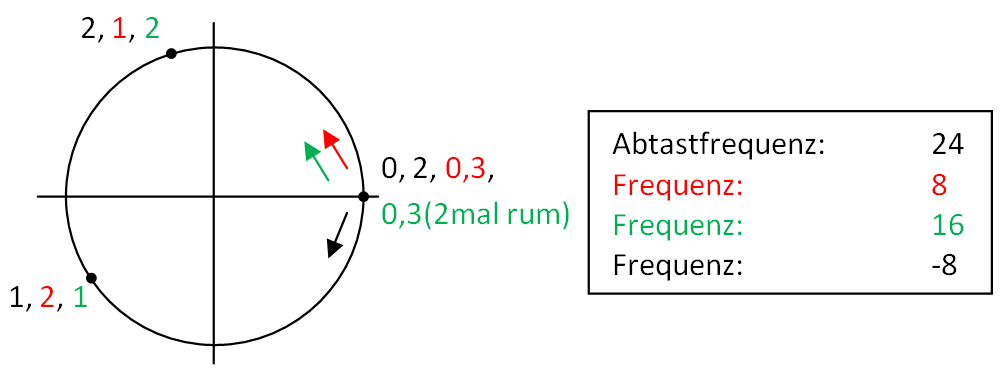
\includegraphics[width=8cm]{./bilder/Alias-effekt.png}
	\end{minipage}
	\begin{minipage}[c]{8cm}
		Summeneigenschaft: $\hat{c_k} = \sum\limits_{m=-\infty}^{\infty} c_{k+mN}$
	\end{minipage}
	%\begin{tabular}{p{8.5cm} p{5cm}}
	%	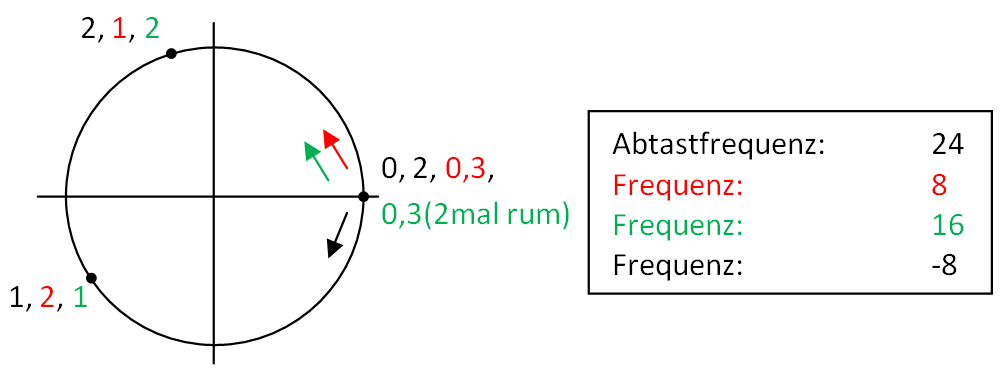
\includegraphics[width=8cm]{./bilder/Alias-effekt.png} & Summeneigenschaft: $\hat{c_k} = \sum\limits_{m=-\infty}^{\infty} c_{k+mN}$
	%\end{tabular}
	

		
		% LaPlace-Transformation
		
\section{Laplace-Transformation}
	$$\boxed{f(t) \; \laplace \; F(s)=\int\limits_0^\infty f(t)e^{-st}dt} \qquad \boxed{ s=\sigma+j\omega}$$\\
	\begin{tabular}{p{0.5cm}p{17.5cm}}
		$\bullet$ & Definitionsbereich nur für kausale Systeme $t\geq 0$\\
		%$\bullet$ & Integrierbar über das Intervall $(0,\infty)$\\
		$\bullet$ & Wachstum kleiner als der von einer Exponentialfunktion\\ 
		$\bullet$ & Gegen"uber $j\omega$ bei der Fourier-Transformation ist bei der
			Laplace-Transformation $s$ verallgemeinert zu $s=\sigma + j\omega$. Das
			bedeutet, dass die Fourier-Transformierte $F(j\omega)$ durch die
			Laplace-Transformation $F(s)$ ausgedr\"uckt werden kann. \\
		$\bullet$ & mit 
		$\begin{cases} 
		\sigma = 0 & \rightarrow \text{Amplitude bleibt konstant} \\ 
		\sigma > 0 & \rightarrow \text{explodiert die Amplitude f\"ur } 0 < t \rightarrow \infty \\
		\sigma < 0 & \rightarrow \text{klingt die Amplidute für } 0 < t \rightarrow \infty \text{ auf $0$ ab} \
		 \end{cases} $ \\   
	\end{tabular}
	
 	\subsection{Eigenschaften der Laplace-Transformation}
  		\renewcommand{\arraystretch}{2}
		\begin{tabular}{|ll|}
	        \hline
	        	Linearität & 
	 			$\alpha\cdot f(t) + \beta\cdot g(t) \; \laplace \; \alpha\cdot F(s) + \beta\cdot
	 			G(s)$ \\
			\hline
	 			"Ahnlichkeit / Streckung im Zeitbereich &
	 			$f(\alpha t) \; \laplace \; \frac{1}{\alpha}F \left (\frac{s}{\alpha} \right ) \quad 0 <\alpha, \alpha \in\mathbb{R}$ \\
	 		\hline
	 		\hline
	 			Faltung im Zeitbereich &
	 			$f(t) \ast g(t) = \int\limits_{0}^{t} f(\tau)g(t-\tau)d\tau \; \laplace \; F(s)
	 			\cdot G(s)$\\
	 		\hline
	 			Faltung im Frequenzbereich &
	 			$f(t) \cdot g(t) \; \laplace \; \frac{1}{2\pi j}\int\limits_{c-j\infty}^{c+j\infty}
	 			F(\xi) G(s-\xi)d\xi$ \\
	 		\hline
	 		\hline
	 			1te Ableitung im Zeitbereich &
	 			$\frac{\partial f(t)}{\partial t} \; \laplace \; sF(s)
	 			-f(0^+)$ \\
	 		\hline
	 			2te Ableitung im Zeitbereich &
	 			$\frac{\partial f(t)}{\partial t} \; \laplace \; s^2F(s)
	 			-sf(0^+) -f'(0^+)$ \\
	 		\hline
	 			nte Ableitung im Zeitbereich &
	 			$\frac{\partial^n f(t)}{\partial t^n} \; \laplace \; s^nF(s)
	 			-s^{n-1}f(0^+)-s^{n-2}\frac{\partial f(0^+)}{\partial t}-\ldots
	 			-s^0\frac{\partial^{n-1} f(0^+)}{\partial t^{n-1}}$ \\
	 		\hline
	 			Ableitung im Frequenzbereich &
		 		$(-t)^n f(t) \; \laplace \;  \frac{\partial^n F(s)}{\partial s^n}$ \\
	 		\hline
	 		\hline
	 			Verschiebung im Zeitbereich nach rechts &
	 			$\sigma(t-a)f(t - a) \; \laplace \; F(s)*e^{-as}$ \\
	 		\hline
				Verschiebung im Zeitbereich nach links &
				$\sigma(t-a)f(t + a) \; \laplace \; e^{as} \cdot [F(s) - \int\limits_0^{a} f(t) \cdot e^{-st} dt]$\\
			\hline
	 			Verschiebung im Frequenzbereich (Dämpfungssatz) &
	 			$f(t)e^{\pm\alpha t} \; \laplace \; F(s\mp\alpha)$ \\
	 		\hline
	 		\hline
	 			Integration im Originalbereich (Sprungantwort)&
	 			$\int\limits_0^t f(u)du \; \laplace \; \frac{1}{s}\cdot F(s)$ \\
	 		\hline
	 			Multiplikation mit $t$ &
	 			$t\cdot f(t)  \; \laplace \; \frac{-\partial F(s)}{\partial s}$ \\
 			\hline
 			\hline
	 			Anfangswert &
	 			$\lim_{t\rightarrow 0^+} f(t) = \lim_{s\rightarrow \infty} sF(s),\text{~wenn
	 			}  \lim_{t\rightarrow 0} f(t)\text{~existiert}.$ \\
 			\hline
	 			Endwert &
	 			$\lim_{t\rightarrow \infty} f(t) = \lim_{s\rightarrow 0} sF(s),\text{~wenn
	 			}  \lim_{t\rightarrow \infty} f(t)\text{~existiert}.$ \\
	 		\hline
       	\end{tabular}
		\renewcommand{\arraystretch}{\arraystretchOriginal}
	
	\subsection{Laplace-Tabelle}
	\renewcommand{\arraystretch}{2}
	\hrule
	\begin{minipage}{9cm}
		\begin{center}
			\begin{tabular}{p{4cm}p{0.75cm}p{3cm}}
				$\sigma \left( t \right)$ & $\; \laplace \;$ & $\dfrac{1}{s}$ \\
				
				$\sigma \left( t \right) \cdot t$ & $\; \laplace \;$ & $\dfrac{1}{s^2}$\\
				
				$\sigma \left( t \right) \cdot t^2$ & $\; \laplace \;$ & $\dfrac{2}{s^3}$\\
				
				$\sigma \left( t \right) \cdot t^n$ & $\; \laplace \;$ & $\dfrac{n!}{s^{n+1}}$\\
				
				$\sigma \left( t \right) \cdot e^{\alpha t}$ & $\; \laplace \;$ &
				$\dfrac{1}{s-\alpha}$\\
				
				$\sigma \left( t \right) \cdot t \cdot e^{\alpha t}$ & $\; \laplace \;$ & $\dfrac{1}{( s - \alpha )^2}$\\
				
				$\sigma \left( t \right)\cdot t^2 \cdot e^{\alpha t}$ &
				$\; \laplace \;$ & $\dfrac{2}{{( s - \alpha )}^3}$\\
				
				$\sigma \left( t \right)\cdot t^n \cdot e^{ \alpha t}$ &
				$\; \laplace \;$ & $\dfrac{n!}{(s-\alpha)^{n+1}}$\\
				
				$\sigma \left( t \right)\cdot \dfrac { 1 - e ^ { - \alpha t } } { \alpha }$ & $\; \laplace \;$ & $\dfrac { 1 } { s ( s + \alpha ) }$\\
				
				$\sigma \left( t \right)\cdot \dfrac {e ^ { - \alpha t }+\alpha t -1 } { \alpha^2 }$ & $\; \laplace \;$ & $\dfrac { 1 } { s^2 ( s + \alpha ) }$\\
				
				$\sigma \left( t \right)\cdot \dfrac {1- e ^ { - \alpha t } - \alpha t e ^ {- \alpha t }}{ \alpha ^2 }$ & $\; \laplace \;$ & $\dfrac { 1 } { s ( s + \alpha )^2 }$\\
					
			\end{tabular}
		\end{center}
	\end{minipage}
\vline
\begin{minipage}{9cm}
\begin{center}
	\begin{tabular}{p{5cm}p{0.75cm}p{3cm}}
	
		$\delta \left( t \right)$ & $\; \laplace \;$ & $1\left( s \right)$ \\
		
		$\delta \left( t - \alpha \right)$ & $\; \laplace \;$ & $e^{- \alpha s}$\\
		
		$\sigma\left( t - \alpha \right)$ & $\; \laplace \;$ & $ \dfrac{1}{s} \cdot e^{- \alpha s}$\\
		
		$\sigma \left( t \right) \cdot \sin \left(\omega t \right)$ & $\; \laplace \;$ &
		$\dfrac{\omega}{s^2 + {\omega^2}}$\\
		
		$\sigma \left( t \right) \cdot \cos \left( \omega t \right)$ & $\; \laplace \;$ &
		$\dfrac{s}{ s^2 + \omega^2}$\\
		
		$\sigma \left( t \right) \cdot  e^{ \alpha t} \cdot \sin \left(\omega t \right)$ & $\; \laplace \;$ 
		& 	$\dfrac{\omega}{(s-a)^2 + {\omega^2}}$\\
		$\sigma \left( t \right) \cdot e^{ \alpha t} \cdot \cos \left( \omega t \right) $ & $\; \laplace \;$ &
		$\dfrac{s-a}{(s-a)^2 + \omega^2}$\\
		
		$\sigma \left( t \right)\cdot t \cdot \dfrac{\sin \left( \alpha t \right)} { 2 \alpha }$ & $\; \laplace \;$ & $\dfrac{s}{ \left(s^ {2}+ \alpha ^{2} \right)^{2}}$ \\
		
		$\sigma \left( t \right)\cdot \dfrac { e ^ { - \alpha t } - e ^ { - \beta t } } { \beta - \alpha }$ & $\; \laplace \;$ & $\dfrac { 1 } { ( s + \alpha ) ( s + \beta ) }$\\
		
		$\sigma \left( t \right)\cdot \dfrac {(\alpha - \beta) +\beta e ^ { - \alpha t } - \alpha e ^ { - \beta t } } { \alpha \beta (\alpha - \beta) }$ & $\; \laplace \;$ & $\dfrac { 1 } {s ( s + \alpha ) ( s + \beta ) }$\\
		
		$\sigma \left( t \right)\cdot \dfrac { e ^ { - \beta t } ( \alpha \cos ( \alpha t ) - \beta \sin ( \alpha t ) ) } { \alpha }$& $\; \laplace \;$ & $\dfrac { s } { ( s + \beta ) ^ { 2 } + \alpha ^ { 2 } }$\\
		
		 
		
		
	\end{tabular}
\end{center}
\end{minipage}


\newpage
\renewcommand{\arraystretch}{\arraystretchOriginal}		
	\subsection{Rücktransformation}
		\subsubsection{Vorgehen}
				1. Kürzen oder vereinfachen \\
				2. Partialbruchzerlegung falls nötig \\
				3. Rücktransformation mittels Laplace-Tabelle \\
				4. $h(t)\hspace{0.2cm}\underline{nicht} < 0$ \\
			
		\subsubsection{Residuensatz}
			Beispiel:\\
			$F(s) = \frac{1}{(s+\alpha)(s+\beta)}, \qquad (0 < \alpha,\beta \in \mathbf{R}, \alpha \neq \beta)$\\
			$f(t) = \frac{1}{2\pi j} \int\limits_{-j\infty}^{j\infty} F(s)e^{st} ds = \sum\limits_{i=1}^k Res(F(s_k)e^{s_kt})$\\
			$=\lim_{s \to -\alpha} ((s+\alpha)F(s)e^{st}) + \lim_{s \to -\beta}((s+\beta)F(s)e^{st})$\\
			$=\frac{e^{-\alpha t}}{\beta - \alpha} + \frac{e^{-\beta t}}{\alpha - \beta} = \frac{e^{-\alpha t}-e^{-\beta t}}{\beta - \alpha}$
			
			
	\subsection{Lösung linearer Differentialgleichungen}
		\begin{minipage}{11.5cm}
			\renewcommand{\arraystretch}{2}
			\begin{tabular}{| l | l |}
				\hline
					Übertragungsfunktion & $G(s) = \frac{1}{p(s)}$\\
					& $g(t) \; \laplace \; G(s)$ \\
				\hline
					Frequenzgang & $G(j\omega) = H(\omega)$ \\
				\hline
					Impulsantwort & $y_{\delta}(t) = g(t) = y_{\sigma}'(t) \; \laplace \; G(s) = \frac{1}{p(s)}=Y_{\delta}(s)$\\
				\hline
					Sprungwantwort & $y_{\sigma}(t)=\int\limits_0^t g(u) du \; \laplace \; \frac{G(s)}{s} = \frac{1}{s \cdot p(s)} = Y_{\sigma}(s)$\\
				\hline
					Eigenschwingung & $\frac{h(s)}{p(s)}$ \\
				\hline
					äussere Erregung & $\frac{F(s)}{p(s)}$ \\
				\hline
					stationärer Zustand & = ungedämpfte Eigenschwingung\\
				\hline
			\end{tabular}
			\renewcommand{\arraystretch}{\arraystretchOriginal}\\
		\end{minipage}
		\begin{minipage}{8cm}
					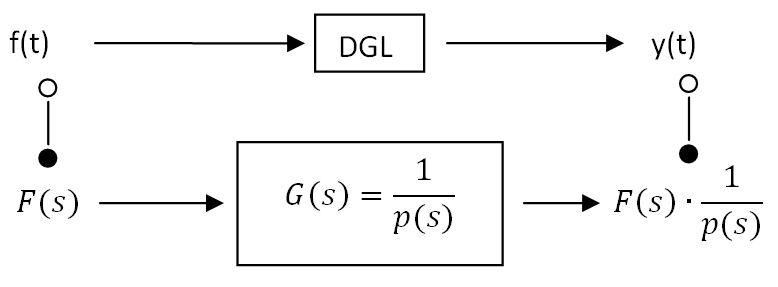
\includegraphics[width=8cm]{./bilder/diffgleichungen2.png} \\
		\end{minipage}
		
		
		\begin{minipage}[l]{16cm}
				\textbf{Beispiel:} $y'' + 8y' + 25y = \sigma{t} \cdot \sin(2t)$ mit $y(0) = 2, y'(0) = -1$\\
				
				$\sin(2t) \; \laplace \; \frac{2}{s^2+4}$ \\ $Y(s)(s^2+8s+25) = 2s+15+\frac{2}{s^2+4}$
				$\Leftrightarrow Y(s) = \frac{2s+15}{s^2+8s+25}+\frac{2}{(s^2+4)(s^2+8s+25)}=
				\underbrace{\frac{2s+15}{s^2+8s+25}}_\text{Eigenschwinung durch Anfangszustand} +
				\underbrace{\frac{As + B}{s^2+4}}_\text{stationärer Zustand} +
				\underbrace{\frac{Cs + D}{s^2+8s+25}}_\text{Eigenschwinung durch Einschalten}$
		\end{minipage}
		\subsubsection{Eigenschwingungen}
			Aus der Eigenschwingung können die Nullstellen des charakteristischen Polynom $p(s)$ 
			direkt abgelesen werden. \\
			\textbf{Beispiel:} \\
			$y(t) = \frac{1}{2} e^{-t} \sin(3t) - \frac{2}{3} e^{-2t} \cos(2t) = 
			\underbrace{\frac{1}{2} e^{\textcolor{red}{-t}} \frac{1}{2j}(e^{\textcolor{red}{3j}t}
			-e^{\textcolor{red}{-3j}t})}_{NS = EW = \textcolor{red}{-1 \pm 3j}} - 
			\underbrace{\frac{2}{3} e^{\textcolor{red}{-2}t} \frac{1}{2}(e^{\textcolor{red}{2j}t}
			+e^{\textcolor{red}{-2j}t})}_{NS = EW = \textcolor{red}{-2 \pm 2j}}$ \\\\
			Damit ist das char. Polynom $p(s) = (s-NS_1)(s-NS_2)\ldots(s-NS_n)$ \\
			Bei mehreren gemessenen Eigenschwingungen werden die char. Polynome multipliziert. \\
			Der stationäre Zustand ist $\lim\limits_{t\rightarrow\infty}y(t) = \frac{1}{p(0)}$ *(Endwertsatz) \\
				
		
	\subsection{Eigenschwingung}
		\begin{minipage}{12cm}
			Spezielle Anfangswerte bei einem System ohne äussere Einflüsse:\\
			$y(0) = 0, y'(0) = 0, \dots , y^{(n-2)} = 0, y^{(n-1)} = 1$\\
			in diesem Fall wird $h(s) = 1$\\
		\end{minipage}
		\begin{minipage}{6cm}
			\begin{math}
				\begin{aligned}
					y(t) \; &\laplace \; Y(s)\\
					y'(t) \; &\laplace \; sY(s) - y_0\\
					y''(t)\; &\laplace \; s^2Y(s) - sy_0 - y'_0\\ 
					y'''(t)\; &\laplace \; s^3Y(s) - s^2y_0 - sy'_0 - y''_0\\ 
					\vdots&\\
					y^{(n)} \; &\laplace \; 
					\underbrace{s^nY(s)}_{Y(s) \cdot p(s)}
					\underbrace{-s^{n-1}y_0 - \dots - y^{(n-1)}}_{h(s)}
				\end{aligned}
			\end{math}
		\end{minipage}
		
		% Diverses
		\newpage
\section{Diverses}
\subsection{Partialbruchzerlegung}
	\[f(x)=\frac{x^2+20x+149}{x^3+4x^2-11x-30} \Rightarrow \; \begin{array}{l}\text{Nenner faktorisieren mit}\\
	\text{Hornerschema, Binom, etc.}\end{array} \Rightarrow
	x^{3}+4x^{2}-11x-30=(x+2)(x^{2}+2x-15)=(x+2)(x+5)(x-3)\] Ansatz:
	\[f(x)=\frac{x^2+20x+149}{x^3+4x^2-11x-30}=\frac{A}{x-3} + \frac{B}{x+2} + \frac{C}{x+5}=
	\frac{A(x+2)(x+5)+B(x-3)(x+5)+C(x-3)(x+2)}{(x-3)(x+2)(x+5)}\]
	Gleichungssystem aufstellen mit beliebigen $x_i$-Werten (am Besten Polstellen oder 0,1,-1 wählen):
	\[\begin{array}{l}x_1=3:\;-9+60+149=A\cdot5\cdot8\;\;\;\Rightarrow A=5\\
	x_2=-2:\;-4-40+149=B(-5)\cdot3\; \Rightarrow B=-7\\
	x_3=-5:\;-25-100+149=C(-8)(-3) \Rightarrow C=1 \end{array} \Rightarrow
	f(x)=\frac{5}{x-3}-\frac{7}{x+2}+\frac{1}{x+5}\] weitere Ansätze für andere
	Typen von Termen: \[f(x)=\frac{5x^2-37x+54}{x^3-6x^2+9x}=\frac{A}{x}+\frac{B}{x-3}+\frac{C}{(x-3)^2}=\frac{A(x-3)^2+Bx(x-3)+Cx}{x(x-3)^2}\]
	\[f(x)=\frac{1,5x}{x^3-6x^2+12x-8}=\frac{A}{x-2}+\frac{B}{(x-2)^2}+\frac{C}{(x-2)^3}=\frac{A(x-2)^2+B(x-2)+C}{(x-2)^3}\]
	\[f(x)=\frac{x^2-1}{x^3+2x^2-2x-12}=\frac{A}{x-2}+\frac{Bx+C}{x^2+4x+6}=\frac{A(x^2+4x+6)+(Bx+C)(x-2)}{(x-2)(x^2+4x+6)}\]

	Variante mit Koeffizientenvergleich: \\
	\[F(s) = \frac{1}{s(s^2+6s+13)} = \frac{A}{s} + \frac{Bs+C}{s^2+6s+13}\]
	\[1 = A(s^2+6s+13) + s(Bs+C) \]
	\[1 = s^2(A+B) + s(C+6A) + 13A \]
	\[\Rightarrow 1 = 13A; (A+B)=0; (C+6A)=0 \]
	\[\Rightarrow A=\frac{1}{13}; B=-\frac{1}{13}; C=-\frac{6}{13}\]

			
\subsection{Hornerschema}
	\begin{minipage}[t]{9cm}
		- Pfeile $\Rightarrow$ Multiplikation\\
		- Zahlen pro Spalte werden addiert\\
		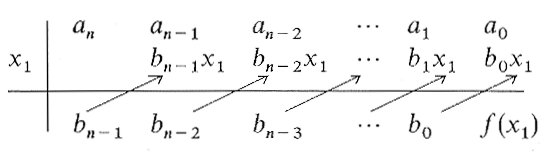
\includegraphics[width=6cm]{./bilder/hornerschema_1.png}\\
		$x_1 \Rightarrow$ Nullstelle (muss erraten werden!!)\\
		oberste Zeile = zu zerlegendes Polynom			
	\end{minipage}
	\begin{minipage}[t]{9cm}
		\textbf{Beispiel:}\\
		$f(x) = x^3-67x-126$\\
		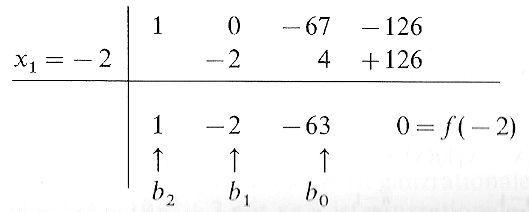
\includegraphics[width=6cm]{./bilder/hornerschema_2.png}\\
		$\Rightarrow f(x) = (x-x_1)(b_2x^2 + b_1x + b_0) = (x+2)(x^2-2x-63)$	
	\end{minipage}

\newpage

\subsection{Schrittfunktion - unit step}
	\begin{minipage}{10cm}
		$u(t) = \sigma(t) =	\begin{cases}
		  		 0 & \text{für } t < 0 \\
		  		 \frac{1}{2} \text{(praxis)}  \text{ oder undef. (math.)} & \text{für } t = 0 \\
		  		 1 & \text{für } t > 0
		  	\end{cases}
		$
		$\sigma(t) \laplace \frac{1}{j\omega} + \pi\delta(\omega) = \Sigma(\omega)$
	\end{minipage}
	\begin{minipage}{8cm}
		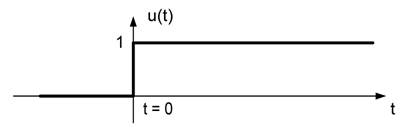
\includegraphics[width=6cm]{./bilder/unitstep.png}
	\end{minipage}

\subsection{Impulsfunktion - dirac delta function}
	\begin{minipage}{10cm}
		\begin{tabular}{l l}
		Definition & $\delta (t)=\begin{cases} 0 & t\ne 0\\\infty & t=0\end{cases}$ \\
				   & $\int\limits_{-\infty}^\infty \delta(t) \, \mathrm dt = 1 $ \\
		Zusammenhang mit der $\sigma$-Funktion & $\frac{d\sigma(t)}{dt}=\delta(t)$ \\
		Abtastung & $\int\limits_{-\infty}^{\infty} \delta(t-t_0)f(t)dt=f(t_0)$ \\
		Transformierte & $\delta(t) \laplace 1(\omega)$ \\
						& $1(t) \laplace 2\pi \cdot \delta(\omega)$ \\
		Faltung & $f(t) \ast \delta(t) = f(t)$ \\
		Ableitung & $\int\limits_{-\infty}^{\infty} \delta^{(k)}(t) \cdot f(t) dt = (-1)^k \cdot f^{(k)}(0)$ \\
		\end{tabular}
	\end{minipage}
	\begin{minipage}{8cm}
		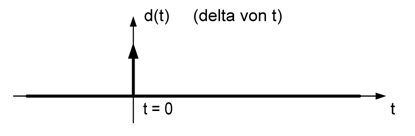
\includegraphics[width=6cm]{./bilder/diracimpulse.png}
	\end{minipage}

	\newpage
		%\section{Riisä Tricks und Merksätze}
\begin{itemize}
  \item $H(s)$ = UTF = Laplace-Transformierte der Impulsantwort ($y_\delta(t)$)
  \item $H(j \omega)$ = Frequenzgang = UTF auf imaginärer Achse
  \item $y_\sigma(t) = \int\limits_0^t y_\delta(u)du$
  \item $\left| \frac{ja + b}{a^2 + b^2} \right| = \sqrt{\frac{1}{a^2 + b^2}}$
  \item Dirac-Funktion: $s(t)\delta(t-t_0) = s(t_0)\delta(t-t_0)$
  \item Antwort eines LTI-Systems auf eine harmonisches Schwingung mit Frequenz $\omega \Rightarrow$ harmonische
  Schwingung mit gleicher Frequenz aber anderer Amplitude und Phase ($\mathcal{L}\{e^{j \omega t}\} = H(\omega) \cdot
  e^{j \omega t}$)
  \item $H(\omega)$ = komplexwertige Funktion der Frequenz $\omega$, die für jede Frequenz $\omega$ die
  Änderung von Amplitude und Phase durch das System speichert = Frequenzgang = Antwort auf harmonische Schwingung
  beliebiger Frequenz
\end{itemize}

		
		% Wichtige Formeln (Idiotenseiten)
		%\subsection{Dreiecksformeln}
\begin{tabular}{lll}
	& \parbox{9.5cm}{
		\textbf{Cosinussatz} \\
		$$c^2 = a^2 + b^2 - 2 \cdot a \cdot b \cdot \cos \gamma$$\\
		\textbf{Sinussatz} \\
		$$\frac{a}{\sin \alpha} = \frac{b}{\sin \beta} = \frac{c}{\sin \gamma} = 2r =
		\frac{u}{\pi}$$
		\textbf{Pythagoras beim Sinus}\\
		$$\sin^2(b)+\cos^2(b)=1 \qquad \tan(b)=\frac{\sin(b)}{\cos(b)}$$}
		
	& \parbox{8cm}{
		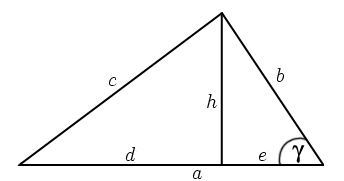
\includegraphics[width=6cm]{./idiotenseite/images/cosinussatz.png}}
\end{tabular}
\begin{center}
	\begin{multicols}{2}
		$\sin \beta = \frac ba =\frac{\text{Gegenkathete}}{\text{Hypotenuse}}$\\
		$\cos \beta = \frac ca =\frac{\text{Ankathete}}{\text{Hypotenuse}}$\\
		$\tan \beta = \frac cb =\frac{\text{Gegenkathete}}{\text{Ankathete}}$\\
		$\cot \beta = \frac cb =\frac{\text{Ankathete}}{\text{Gegenkathete}}$\\
	\end{multicols}
\end{center}

	
\subsection{Funktionswerte für Winkelargumente}
	\begin{minipage}{5cm}	
	\begin{tabular}[c]{|p{0.5cm}|p{0.4cm}||p{0.5cm}|p{0.5cm}|p{0.7cm}|}
	    	\hline
			deg & rad & sin & cos & tan$^-1$\\
			\hline
			0\symbol{23} & 0 & 0 & 1 & 0\\
			\hline
			30\symbol{23} & $\frac{\pi}{6}$ & $\frac{1}{2}$ & $\frac{\sqrt{3}}{2}$ &
			$\frac{1}{\sqrt{3}}$\\
			\hline
			45\symbol{23} & $\frac{\pi}{4}$ & $\frac{\sqrt{2}}{2}$ & $\frac{\sqrt{2}}{2}$
			& 1\\
			\hline
			60\symbol{23} & $\frac{\pi}{3}$ & $\frac{\sqrt{3}}{2}$ & $\frac{1}{2}$ &
			$\sqrt{3}$\\
			\hline			
	\end{tabular} \\
\end{minipage}
\begin{minipage}{14cm}
	\begin{multicols}{3}	
	\begin{tabular}[c]{|p{0.7cm}|p{0.7cm}||p{0.7cm}|p{0.7cm}|}
	    	\hline
			deg & rad & sin & cos\\
			\hline
			90\symbol{23} & $\frac{\pi}{2}$ & 1 & 0\\
			\hline	
			120\symbol{23} & $\frac{2\pi}{3}$ & $\frac{\sqrt{3}}{2}$ & $-\frac{1}{2}$ \\
			\hline
			135\symbol{23} & $\frac{3\pi}{4}$ & $\frac{\sqrt{2}}{2}$ & $-\frac{\sqrt{2}}{2}$\\
			\hline
			150\symbol{23} & $\frac{5\pi}{6}$ & $\frac{1}{2}$ & $-\frac{\sqrt{3}}{2}$\\
			\hline
	\end{tabular} \\
	
	\begin{tabular}[c]{|p{0.7cm}|p{0.7cm}||p{0.7cm}|p{0.7cm}|}
	  	\hline
		deg & rad & sin & cos\\
		\hline
		180\symbol{23} & $\pi$ & 0 & -1\\
		\hline	
		210\symbol{23} & $\frac{7\pi}{6}$ & $-\frac{1}{2}$ & $-\frac{\sqrt{3}}{2}$\\
		\hline
		225\symbol{23} & $\frac{5\pi}{4}$ & $-\frac{\sqrt{2}}{2}$ & $-\frac{\sqrt{2}}{2}$\\
		\hline
		240\symbol{23} & $\frac{4\pi}{3}$ & $-\frac{\sqrt{3}}{2}$ & $-\frac{1}{2}$\\
		\hline
	\end{tabular} \\
	
	\begin{tabular}[c]{|p{0.7cm}|p{0.7cm}||p{0.7cm}|p{0.7cm}|}
    	\hline
		deg & rad & sin & cos\\
		\hline
		270\symbol{23} & $\frac{3\pi}{2}$ & -1 & 0\\
		\hline	
		300\symbol{23} & $\frac{5\pi}{3}$ & $-\frac{\sqrt{3}}{2}$ & $\frac{1}{2}$\\
		\hline
		315\symbol{23} & $\frac{7\pi}{4}$ & $-\frac{\sqrt{2}}{2}$ & $\frac{\sqrt{2}}{2}$\\
		\hline
		330\symbol{23} & $\frac{11\pi}{6}$ & $-\frac{1}{2}$ & $\frac{\sqrt{3}}{2}$\\
		\hline
	\end{tabular}					
\end{multicols}
\end{minipage}

\begin{minipage}{13cm}
	\subsection{Periodizität}
	$\cos(a+k\cdot2\pi)=\cos(a) \qquad \sin(a+k\cdot2\pi)=\sin(a) \qquad
	(k \in \mathbb{Z})$
	\subsection{Quadrantenbeziehungen}
	\begin{tabbing}
    	xxxxxxxxxxxxxxxxxxxxxxxxxxxxxxxxxx \= \kill
	  	$\sin(-a)=-\sin(a)$ \> $\cos(-a)=\cos(a)$\\
		$\sin(\pi - a)=\sin(a)$ \> $\cos(\pi - a)=-\cos(a)$\\
		$\sin(\pi + a)=-\sin(a)$ \> $\cos(\pi +a)=-\cos(a)$\\
		$\sin\left(\frac{\pi}{2}-a \right)=\sin\left(\frac{\pi}{2}+a \right)=\cos(a)$ \>
		$\cos\left(\frac{\pi}{2}-a \right)=-\cos\left(\frac{\pi}{2}+a \right)=\sin(a)$  
    \end{tabbing}
\end{minipage}
\begin{minipage}{5cm}
	

\subsection{Ableitungen}

\begin{tikzpicture}
	[	inner sep = 2mm,
		sin/.style={rectangle,minimum width=1.2cm,minimum height=1cm,rounded corners=5pt,draw=black,top color=green!20!black!50},
		abl/.style={rectangle}
	]
	\node at (1.2,0) (sin1) [sin] {$\sin$};
	\node at (0,-1.2) (cos2) [sin] {$-\cos$};
	\node at (1.2,-2.4) (sin2) [sin] {$-\sin$};
	\node at (2.4,-1.2) (cos1) [sin] {$\cos$};
	
	\draw[thick,black,->] (sin1.east) .. controls +(right:0.6cm) and +(up:0.6cm) ..  (cos1.north)
	node [pos=0.5,above](abl) {$\frac{d}{dx}$};
	\draw[thick,black,->] (cos1.south) .. controls +(down:0.6cm) and +(right:0.6cm) .. (sin2.east)
	node [pos=0.5,below](abl) {$\frac{d}{dx}$};
	\draw[thick,black,->] (sin2.west) .. controls +(left:0.6cm) and +(down:0.6cm) .. (cos2.south)
	node [pos=0.5,below](abl) {$\frac{d}{dx}$};
	\draw[thick,black,->] (cos2.north) .. controls +(up:0.6cm) and +(left:0.6cm) .. (sin1.west)
	node [pos=0.5,above](abl) {$\frac{d}{dx}$};
\end{tikzpicture}
\end{minipage}
\begin{multicols}{2}
	\subsection{Additionstheoreme}
	$\sin(a \pm b)=\sin(a) \cdot \cos(b) \pm \cos(a) \cdot \sin(b)$\\
	$\cos(a \pm b)=\cos(a) \cdot \cos(b) \mp \sin(a) \cdot \sin(b)$\\	
	$\tan(a \pm b)=\dfrac{\tan(a) \pm \tan(b)}{1 \mp \tan(a) \cdot \tan(b)}$
	\columnbreak
	
	\subsection{Doppel- und Halbwinkel}	
	$\sin(2a)=2\sin(a)\cos(a)$\\
	$\cos(2a)=\cos^2(a)-\sin^2(a)=2\cos^2(a)-1=1-2\sin^2(a)$\\
	$\cos^2 \left(\frac{a}{2}\right)=\frac{1+\cos(a)}{2} \qquad
	\sin^2 \left(\dfrac{a}{2}\right)=\frac{1-\cos(a)}{2}$
\end{multicols}
\begin{multicols}{2}
	\subsection{Produkte}
		$\sin(a)\sin(b)=\frac{1}{2}(\cos(a-b)-\cos(a+b))$\\
		$\cos(a)\cos(b)=\frac{1}{2}(\cos(a-b)+\cos(a+b))$\\
		$\sin(a)\cos(b)=\frac{1}{2}(\sin(a-b)+\sin(a+b))$\\
	\subsection{Euler-Formeln} 

	$\sin(x) = \frac{1}{2j} \left(e^{jx} - e^{-jx}\right) \qquad
	\cos(x) = \frac{1}{2} \left(e^{jx} + e^{-jx}\right)$ \\
	$e^{x+jy} = e^x \cdot e^{jy} = e^x \cdot \left(\cos(y) + j\sin(y)\right)$ \\
	$e^{j\pi} = e^{-j\pi} = -1$ \\
	\columnbreak
	
	\subsection{Summe und Differenz}
		$\sin(a)+\sin(b)=2 \cdot \sin \left(\frac{a+b}{2}\right) \cdot
		\cos\left(\frac{a-b}{2}\right)$\\
		$\sin(a)-\sin(b)=2 \cdot \sin \left(\frac{a-b}{2}\right) \cdot
		\cos\left(\frac{a+b}{2}\right)$\\
		$\cos(a)+\cos(b)=2 \cdot \cos \left(\frac{a+b}{2}\right) \cdot
		\cos\left(\frac{a-b}{2}\right)$\\
		$\cos(a)-\cos(b)=-2 \cdot \sin \left(\frac{a+b}{2}\right) \cdot
		\sin\left(\frac{a-b}{2}\right)$\\
		$\tan(a) \pm \tan(b)=\dfrac{\sin(a \pm b)}{\cos(a)\cos(b)}$\\
\end{multicols}

		%\section{Idiotenseite}
%\subsection{Diverses}
\begin{tabbing}
	xxxxxxxxxxxxxxxxxxxxxxxxxxxx \= xxxxxxxxxxxxxxxxxxxxxxxxxxxxxx \= \kill
 	$f'(z) = \lim \limits_{\Delta z \rightarrow 0} \frac{f(z + \Delta z) -
	f(z)}{\Delta z}$ \> $(a + b)^n = \sum_{k=0}^{n} \binom n k a^{n-k} \cdot b^k$ \>
	$(a \pm b)^3 =a^3 \pm  3 a^{2} b + 3 a b^2 \pm b^3 $\\ \\
	$x_{1,2} = \dfrac{-b \pm \sqrt{b^2 - 4ac}}{2a}$ \> $\binom n k = \dfrac{n!}{k!
	\cdot (n-k)!}$ \> $(a \pm b)^4 =a^4 \pm  4 a^{3} b + 6a^2b^2 \pm 4 a b^3 +
	b^4$\\
\end{tabbing}
%\subsection{Reihenentwicklungen}
\begin{tabular}{llll}
\textbf{Geometrische Reihe}
	& $\sum\limits_{n=0}^{\infty} x^n$ 
	& $= \dfrac{1}{1-x}$
	& $|x| < 1$ \\
	
	& $\sum\limits_{k=0}^{\infty} k \, x^k$ & $= x \sum\limits_{k=1}^{\infty} k \,
	x^{k-1} = \dfrac{x}{(1-x)^2} $ 
	& $x \neq 1$ \\
\textbf{Binominalreihe} 
	& $\sum\limits_{n=0}^\infty \binom{\alpha}{n} x^n $ &$= (1+x)^\alpha$
	& $x \in (-1,1)$ \\
\textbf{E-Funktion}
	& $\sum\limits_{k = 0}^{\infty} \dfrac{x^k}{k!}$ &$ = e^x$
	& 
\end{tabular}

		
		% Integraltabelle
		%\section{Integralrechnung}
Partielle Integration: $\int u(x) v'(x) dx = u(x)v(x) - \int u'(x) v(x) dx$

\subsection{Einige wichtige Integrale}
  	\renewcommand{\arraystretch}{2}
	\begin{tabular}{|l|l|}
    	\hline
    	$\int \sin(x)dx=-\cos(x)$ & $\int \sin(a+bx)dx=-\frac1b \cos(a+bx)$\\
    	\hline
	  	$\int \sin^2(x)dx=-\frac14 \sin(2x)+\frac x2$ 
    	& $\int
    	e^{ax+c}\sin(bx+d)dx=\frac{e^{ax+c}}{a^2+b^2}(a\sin(bx+d)-b\cos(bx+d))$\\
    	\hline
    	$\int \cos(x)dx=\sin(x)$ & $\int \cos(a+bx)dx=\frac1b \sin(a+bx)$\\
    	\hline
	  	$\int \cos^2(x)dx=\frac14 \sin(2x)+\frac x2$ 
    	& $\int
    	e^{ax+c}\cos(bx+d)dx=\frac{e^{ax+c}}{a^2+b^2}(a\cos(bx+d)+b\sin(bx+d))$\\
    	\hline
    	$\int e^x dx=e^x$ & $\int e^{ax}dx=\frac1a e^{ax}$\\
    	\hline
    	$\int xe^{ax}dx=\frac{1}{a^2} e^{ax}(ax-1)$ & $\int x^2 e^{ax} dx =
    	e^{ax}\left( \frac{x^2}{a} - \frac{2x}{a^2} + \frac{2}{a^3}\right)$ \\
    	\hline
    	$\int x^n e^{ax} dx = \frac{1}{a} x^n e^{ax} - \frac{n}{a} \int x^{n-1}
    	e^{ax} dx$ & \\
    	\hline
    \end{tabular}

\section{Differentialrechnung}
\subsection{Einige wichtige Differentiale}
\begin{multicols}{2}
	\begin{tabular}{|l|l||l|l|}
    	\hline
    	\textbf{Funktion} & \textbf{Ableitung} & \textbf{Funktion} &
    	\textbf{Ableitung}\\
    	\hline
    	\hline
    	$C \text{ (Konstante)}$ & $0$ & $x$ & $1$\\
    	\hline
    	$x^n$ & $nx^{n-1}$ & $\frac1x$ & $-\frac{1}{x^2}$\\
    	\hline
    	$\sqrt{x}$ & $\frac{1}{2\sqrt{x}}$ & $e^x$ & $e^x$\\
    	\hline
    	$e^{bx}$ & $be^{bx}$ & $a^x$ & $a^x \ln(a)$\\
    	\hline
    	$\ln(x)$ & $\frac1x$ & $\sin(x)$ & $\cos(x)$\\
    	\hline
    	$\cos(x)$ & $-\sin(x)$ & $\ln[f(x)]$ & $\frac{f^{'}(x)}{f(x)}$\\
    	\hline	
    \end{tabular}
\columnbreak  	
\subsection{Aufgabenbeispiel}
$f(t) =\sum_{k=0}^{\infty}\delta (t-k\pi) \cdot cos(t)$ \\
$ = \sum_{k=0}^{\infty} = \delta (t-k\pi) \cdot cos(\pi t)  \\
\; \laplace \; 
F(s) = \sum_{k=0}^{\infty} (-1)^k(e^{-k\pi s}) \\
= \sum_{k=0}^{\infty} (-1)^k(e^{-\pi s})^k$ 
\\ \\
Die Summenformel der geometrischen Reihe liefert: \\
$F(s) = \dfrac{e^{-\pi s}}{1 +e^{-\pi s}}$ \\

\end{multicols}
\renewcommand{\arraystretch}{\arraystretchOriginal} 
		%\begin{sidewaystable}
\subsection{Einige unbestimmte Integrale\formelbuch{1074}}
\label{unbestimmte_integrale}
\begin{tabular}{|p{12cm}|p{13cm}|}
  \hline
  
    $ \int dx=x+C $ &
     $ \int{x^\alpha}dx=\frac{x^{\alpha+1}}{\alpha+1}+C,\ x \epsilon \mathbb
    R ^+,\ \alpha \epsilon \mathbb R \backslash \{ -1 \} $ \\\hline
     $ \int{\frac{1}{x}}dx=\ln \left| x \right| + C,\ x\neq0 $ &
     $ \int{e^x}dx=e^x+C $ \\\hline
     $ \int{a^x}dx=\frac{a^x}{\ln{a}}+C,\ a \epsilon \mathbb 
    R^+\backslash\{1\} $ &
     $ \int{ \sin{x}} dx = -\cos{x} + C $ \\\hline
     $ \int{\cos{x}} dx = \sin{x} + C $ &
     $ \int{\frac{dx}{\sin^2x}}=-\cot{x}+C,\ x\neq k\pi\ \mathrm{mit}\ k
    \epsilon \mathbb Z $ \\\hline
     $ \int{\frac{dx}{\cos^2x}}=\tan{x}+C,\ x\neq\frac{\pi}{2}+k\pi\
    \mathrm{mit} k \epsilon \mathbb Z $ & 
    
    %10. :
     $ \int{\sinh{x}}dx = \cosh{x}+C $ \\ \hline
     $ \int{\cosh{x}}dx = \sinh{x}+C $ &
     $ \int{\frac{dx}{\sinh^2x}}=-\coth{x}+C,\ x\neq0 $ \\\hline
     $ \int{\frac{dx}{\cosh^2x}}=\tanh{x}+C $ &
     $ \int{\frac{dx}{ax+b}} = \frac{1}{a}\ln \left|ax + b\right| + C,\
    a\neq 0,x\neq-\frac{b}{a} $ \\\hline
     $ \int{\frac{dx}{a^2x^2+b^2}}=\frac{1}{ab}\arctan{\frac{a}{b}x}+C,\
    a\neq0,\ b\neq0 $ &
     $
    \int{\frac{dx}{a^2x^2-b^2}}=\frac{1}{2ab}\ln{\left|\frac{ax-b}{ax+b}\right|}+C,\
    a\neq0,\ b\neq0,\ x\neq\frac{b}{a},\ x\neq-\frac{b}{a} $ \\\hline
     $
    \int{\sqrt{a^2x^2+b^2}}dx=\frac{x}{2}\sqrt{a^2x^2+b^2}+\frac{b^2}{2a}\ln{(ax+\sqrt{a^2x^2+b^2})}+C,\
    a\neq0,\ b\neq0 $ &
     $
    \int{\sqrt{a^2x^2-b^2}}dx=\frac{x}{2}\sqrt{a^2x^2-b^2}-\frac{b^2}{2a}\ln\left|ax+\sqrt{a^2x^2-b^2}\right|+C,\
    a\neq0,\ b\neq0,a^2x^2\geqq b^2$ \\\hline
     $
    \int\sqrt{b^2-a^2x^2}dx=\frac{x}{2}\sqrt{b^2-a^2x^2}+\frac{b^2}{2a}\arcsin\frac{a}{b}x+C,\
    a\neq0,\ b\neq0,\ a^2x^2\leqq b^2 $ &
    %20.:
     $
    \int\frac{dx}{\sqrt{a^2x^2-b^2}}=\frac{1}{a}\ln(ax+\sqrt{a^2x^2+b^2})+C,\
    a\neq0,\ b\neq0 $ \\\hline
     $
    \int\frac{dx}{\sqrt{a^2x^2-b^2}}=\frac{1}{a}\ln\left|ax+\sqrt{a^2x^2-b^2}\right|+C,\
    a\neq0,\ b\neq0,\ a^2x^2>b^2 $ &
     $ \int\frac{dx}{\sqrt{b^2-a^2x^2}}=\frac{1}{a}\arcsin\frac{a}{b}x+C,\
    a\neq0,\ b\neq0,\ a^2x^2<b^2 $ \\\hline
     Die Integrale $\int\frac{dx}{X}, \int\sqrt{X}dx,
    \int\frac{dx}{\sqrt{X}}$ mit $X=ax^2+2bx+c,\ a\neq0 $ werden durch 
    die Umformung $X=a(x+\frac{b}{a})^2+(c-\frac{b^2}{a}) $ und die
    Substitution $ t=x+\frac{b}{a} $ in die oberen 4 Zeilen
    transformiert. & $ \int\frac{xdx}{X}=\frac{1}{2a}\ln\left|X\right|-\frac{b}{a}\int\frac{dx}{X},\
    a\neq0,\ X=ax^2+2bx+c $ \\\hline
     $ \int\sin^2axdx=\frac{x}{2}-\frac{1}{4a}\cdot\sin2ax+C,\ a\neq0 $ &
     $ \int\cos^2axdx=\frac{x}{2}+\frac{1}{4a}\cdot\sin2ax+C,\ a\neq0 $ \\\hline
     $ \int\sin^naxdx=-\frac{sin^{n-1}ax\cdot\cos
    ax}{na}+\frac{n-1}{n}\int\sin^{n-2}axdx,\ n \epsilon \mathbb N,\ a\neq0 $ &
     $ \int\cos^naxdx=\frac{\cos^{n-1}ax\cdot\sin
    ax}{na}+\frac{n-1}{n}\int\cos^{n-2}axdx,\ n\epsilon \mathbb N,\ a\neq0 $
    \\\hline
     $ \int\frac{dx}{\sin ax} =
    \frac{1}{a}\ln\left|\tan\frac{ax}{2}\right|+C,\ a\neq0,\ x\neq
    k\frac{\pi}{a}\ \mathrm{mit}\ k\epsilon\mathbb Z$ &
    %30.:
     $ \int\frac{dx}{\cos
    ax}=\frac{1}{a}\ln\left|\tan(\frac{ax}{2}+\frac{\pi}{4})\right|+C,\ a\neq0,\
    x\neq\frac{\pi}{2a}+k\frac{\pi}{a}\ \mathrm{mit}\ k\epsilon\mathbb Z $
    \\\hline
     $\int\tan axdx=-\frac{1}{a}\ln\left|\cos ax\right|+C,\ a\neq0,\
    x\neq\frac{\pi}{2a}+k\frac{\pi}{a} \mathrm{mit}\ k\epsilon\mathbb Z$ &
     $\int\cot axdx=\frac{1}{a}\ln\left|\sin ax\right|+C,\ a\neq0,\ x\neq
    k\frac{\pi}{a} \mathrm{mit} k\epsilon\mathbb Z $ \\ \hline
     $ \int x^n\sin axdx=-\frac{x^n}{a}\cos ax+\frac{n}{a}\int x^{n-1}\cos
    axdx,\ n\epsilon\mathbb N,\ a\neq0 $ &
    $ \int x^n\cos axdx=\frac{x^n}{a}\sin ax-\frac{n}{a}\int x^{n-1}\sin
    axdx,\ n\epsilon\mathbb N,\ a\neq0 $ \\ \hline
     $ \int x^ne^{ax}dx=\frac{1}{a}x^ne^{ax}-\frac{n}{a}\int
    x^{n-1}e^{ax}dx,\ n\epsilon\mathbb N,\ a\neq0 $ &
     $ \int e^{ax}\sin bxdx=\frac{e^{ax}}{a^2+b^2}(a\sin bx-b\cos bx)+C,\
    a\neq0,\ b\neq0 $  \\ \hline
     $ \int e^{ax}\cos bxdx=\frac{e^{ax}}{a^2+b^2}(a\cos bx + b\sin bx)+C,\
    a\neq0,\ b\neq0 $ &
     $ \int\ln x dx = x(\ln x-1)+C,\ x\epsilon\mathbb R^+ $ \\ \hline
     $ \int x^\alpha \cdot \ln xdx =
    \frac{x^{\alpha+1}}{(\alpha+1)^2}\lbrack(\alpha+1)\ln x-1\rbrack + C,\
    x\epsilon\mathbb R^+,\ \alpha\epsilon\mathbb R\backslash\{-1\} $ & \\ \hline
    %FF1 Seite 496
    
\end{tabular}
\end{sidewaystable}

\end{document}